%%% ====================== %%%
%%%      INTRODUCTION      %%%
%%% ====================== %%%

% FIGURE 0-01 - LENGTH SCALES IN ATMOSPHERIC SCIENCES

\begin{figure}
\centering
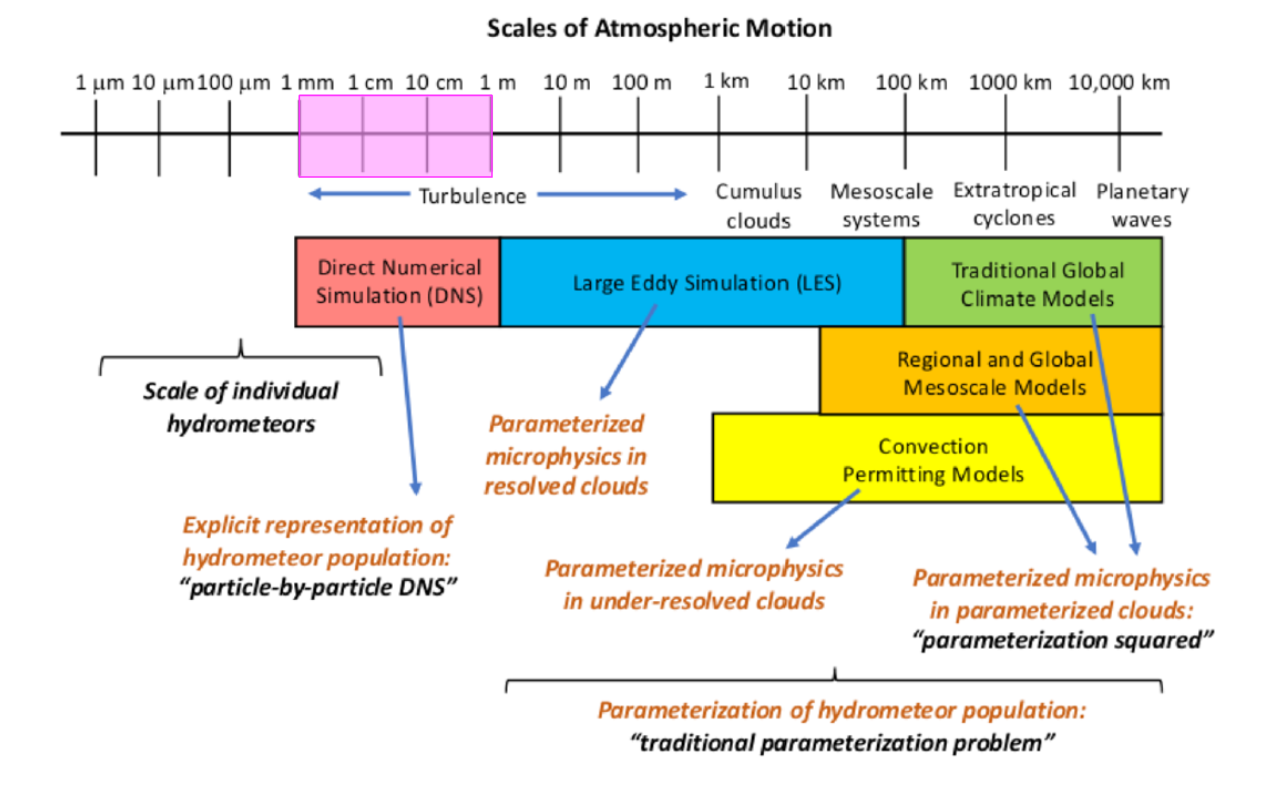
\includegraphics[width=13cm]{figures/0-01_atmo-scales.png}
\caption{
Hierarchy of atmospheric models and the scales of atmospheric motion reproduced from \textcite{Morrison2020} with author's permission.
Coloured rectangles represent types of simulations commonly used when working with respective length scales, and comments emphasise transition from directly resolving most elements of the model (left) to including more and more parameterisations with the increase of scale (right).
Magenta rectangle positioned on the axis was added to emphasise range of scales that corresponds to simulations discussed in this thesis.}
\label{fig:atmo-scales}
\end{figure}



%%% =================== %%%
%%%      CHAPTER 1      %%%
%%% =================== %%%

% FIGURE 1-01 - DETERMINISTIC FORCING ENERGY SPECTRUM

\begin{figure}
\centering
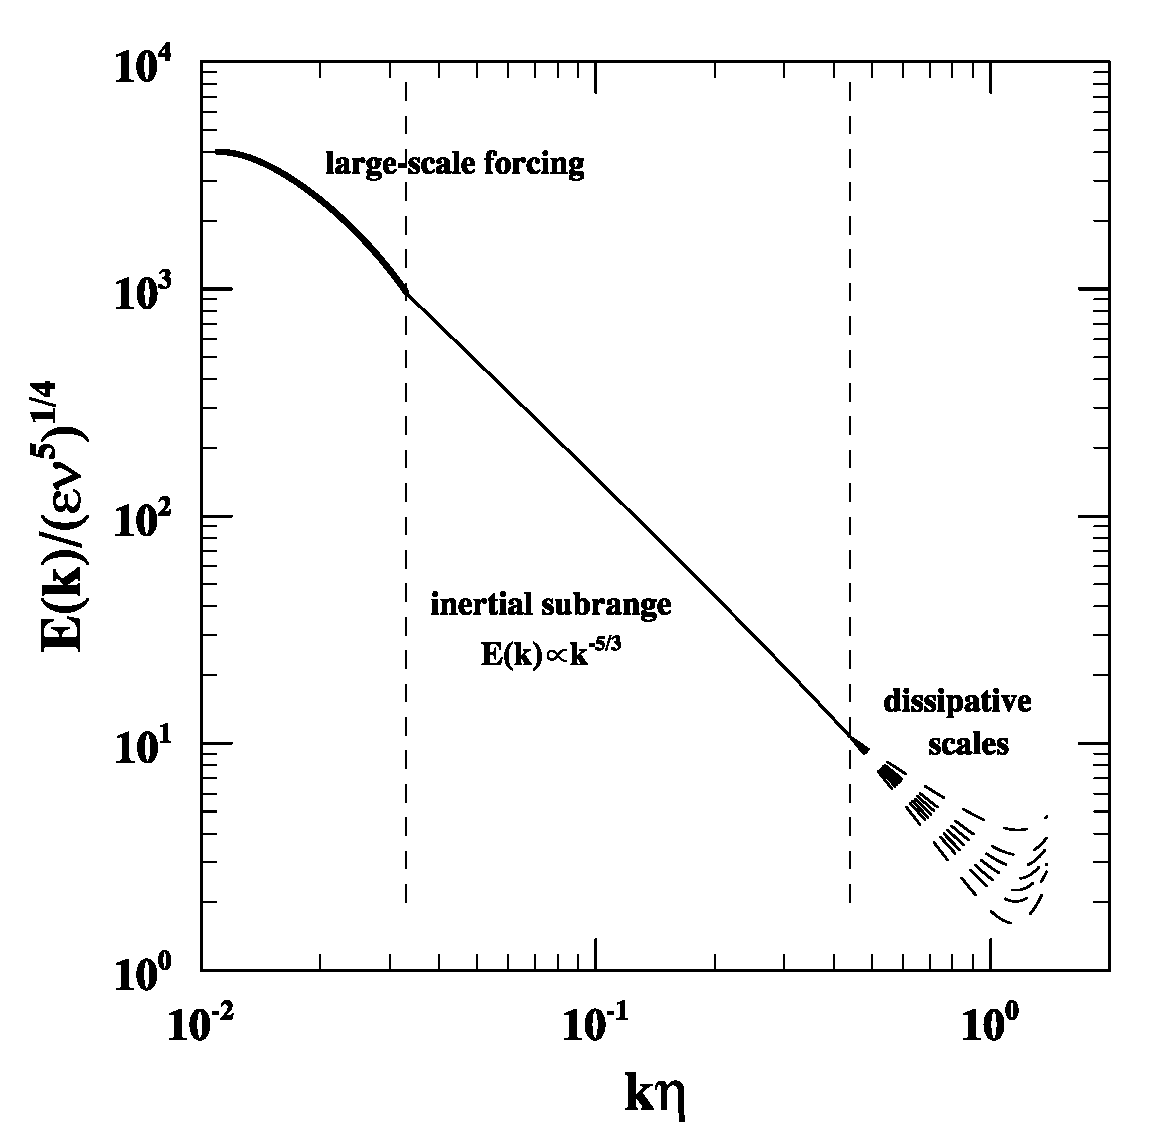
\includegraphics[width=10cm]{figures/1-01_forcing.pdf}
\caption{
The basic idea of deterministic forcing scheme: energy is supplied on large scales by fixing it for small wavenumbers (bold line), then it is transferred following Kolmogorov energy cascade ($E(k) \propto k^{-5/3}$) in inertial subrange, to finally reach smallest dissipative eddies represented by largest resolved wavenumbers (when $k_{\max} \eta \sim 1 = 10^0$, diverging dashed lines) that have largest influence on measured particle statistics at contact distances.
Both axes are using standard normalisations (see Section \ref{ssc:ch2.flow.spec}) and logarithmic scale, that makes $k^{-5/3}$ curves appear as straight lines.}
\label{fig:forcing}
\end{figure}

% FIGURE 1-02 - GRID SIZES IN DNS VS LES

\begin{figure}
\centering
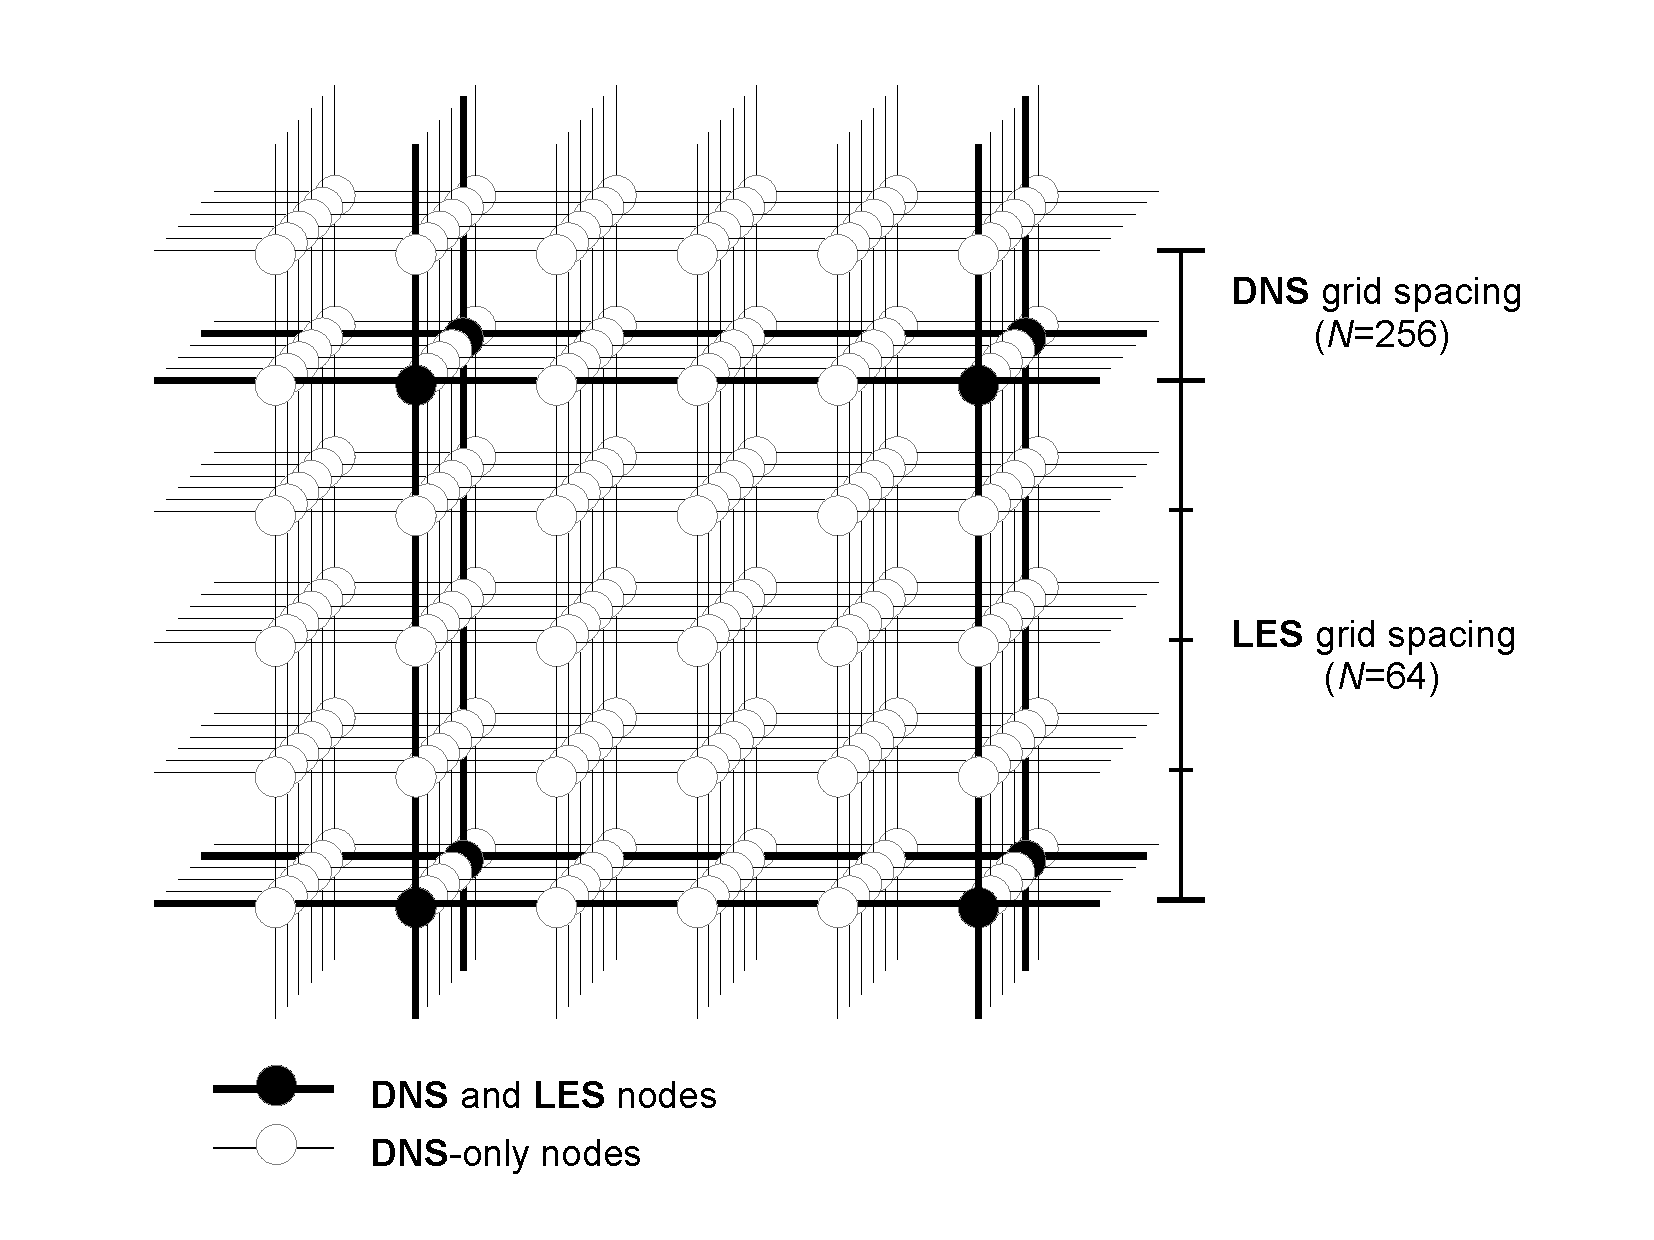
\includegraphics[width=17cm]{figures/1-02_dns-les-grids.pdf}
\caption{
Conceptual juxtaposition of computational grids for DNS and LES.
In LES, the subgrid-scale modelling parameterises small-scale turbulence that is directly resolved by $4 \times 4 \times 4$ block of cells in DNS.
}
\label{fig:dns-les-grids}
\end{figure}

% FIGURE 1-03 - PROJECTION ONTO NEIGHBOURING NODES

\begin{figure}
\centering
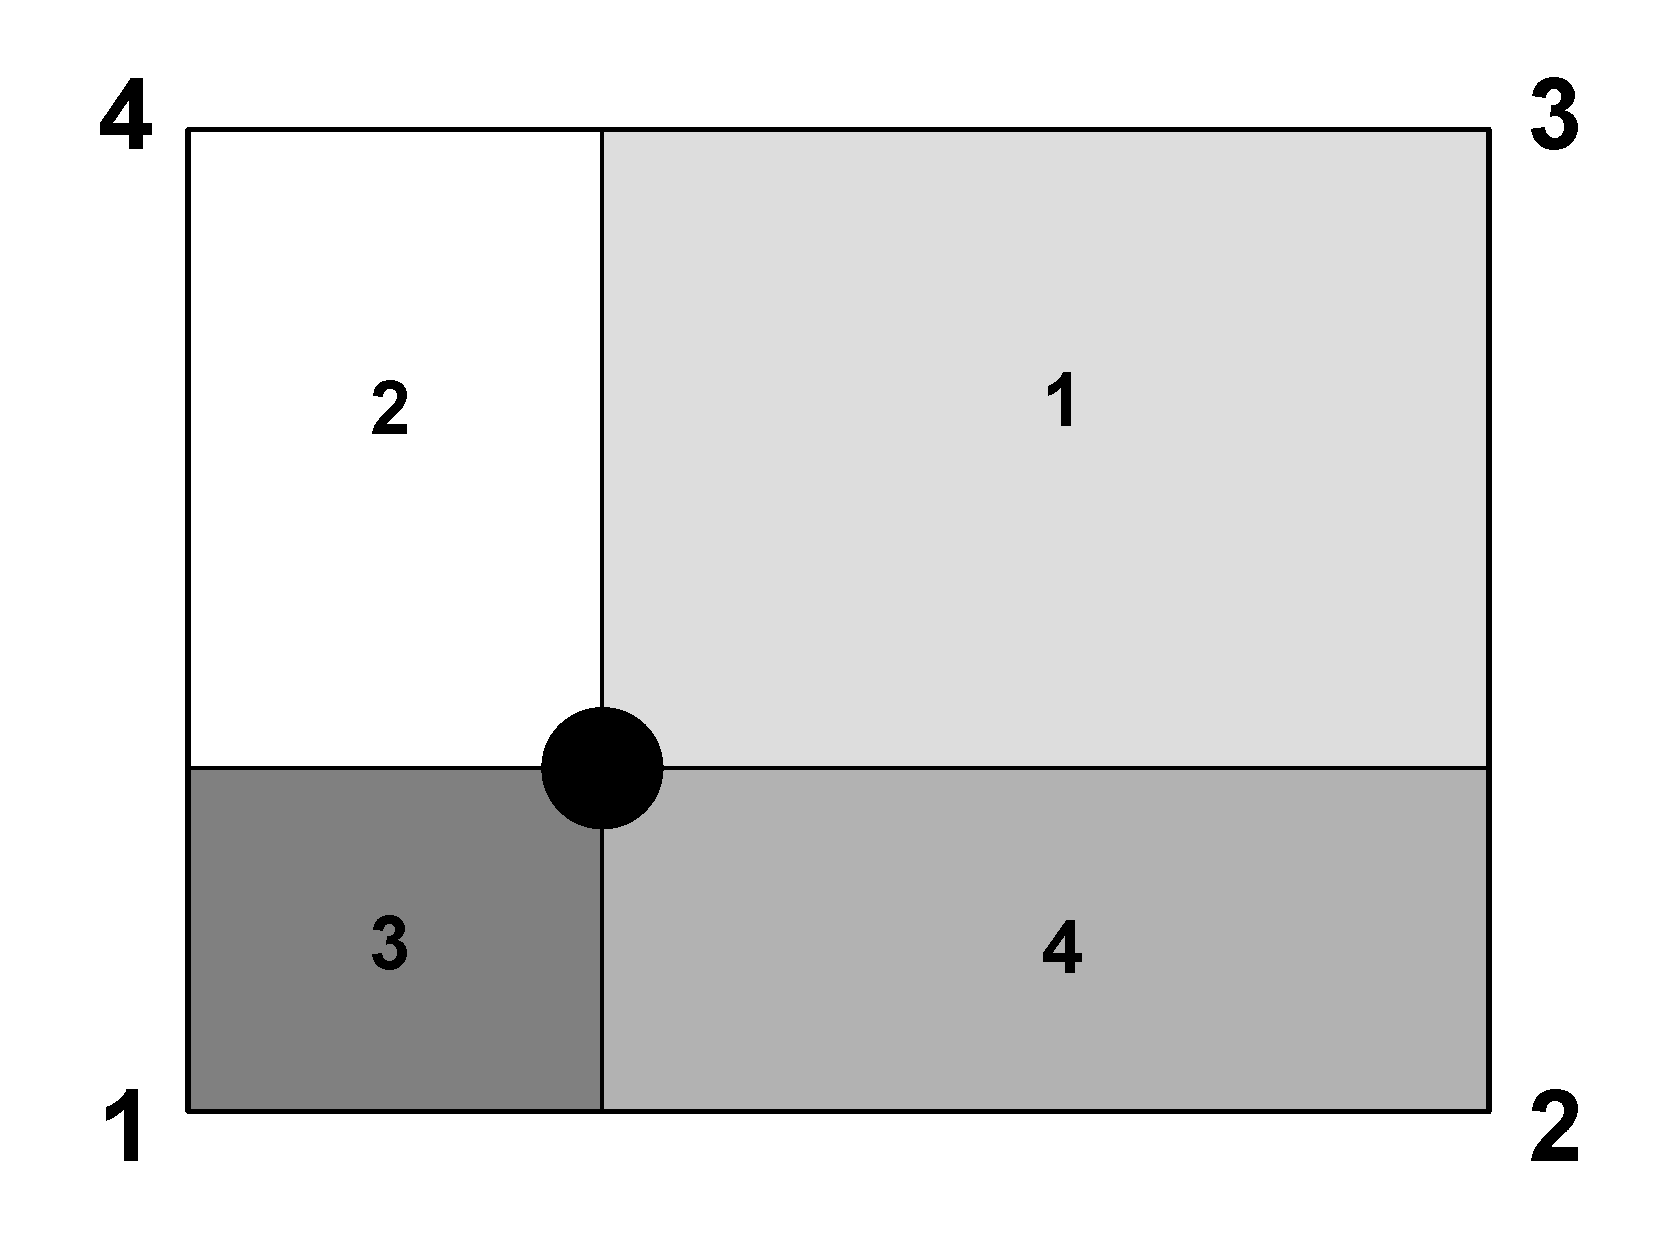
\includegraphics[width=8cm]{figures/1-03_pnn.pdf}
\caption{
Projection onto neighbouring nodes (PNN; simplified illustration for 2D case).
The contribution of the particle momentum to the fluid momentum at a grid node depends on the separation distance.
For example, the particle force may be projected onto neighbouring nodes using weights that are proportional to cell areas (or volumes in 3D case).
Here, the fluid flow at grid node $1$ is affected by a fraction of the particle Stokes drag proportional to the area with marker $1$, and so on.
Based on \textcite[Fig. 1 therein]{Garg2007}.}
\label{fig:pnn}
\end{figure}

% FIGURE 1-04 - 2D DOMAIN DECOMPOSITION

\begin{figure}
\centering
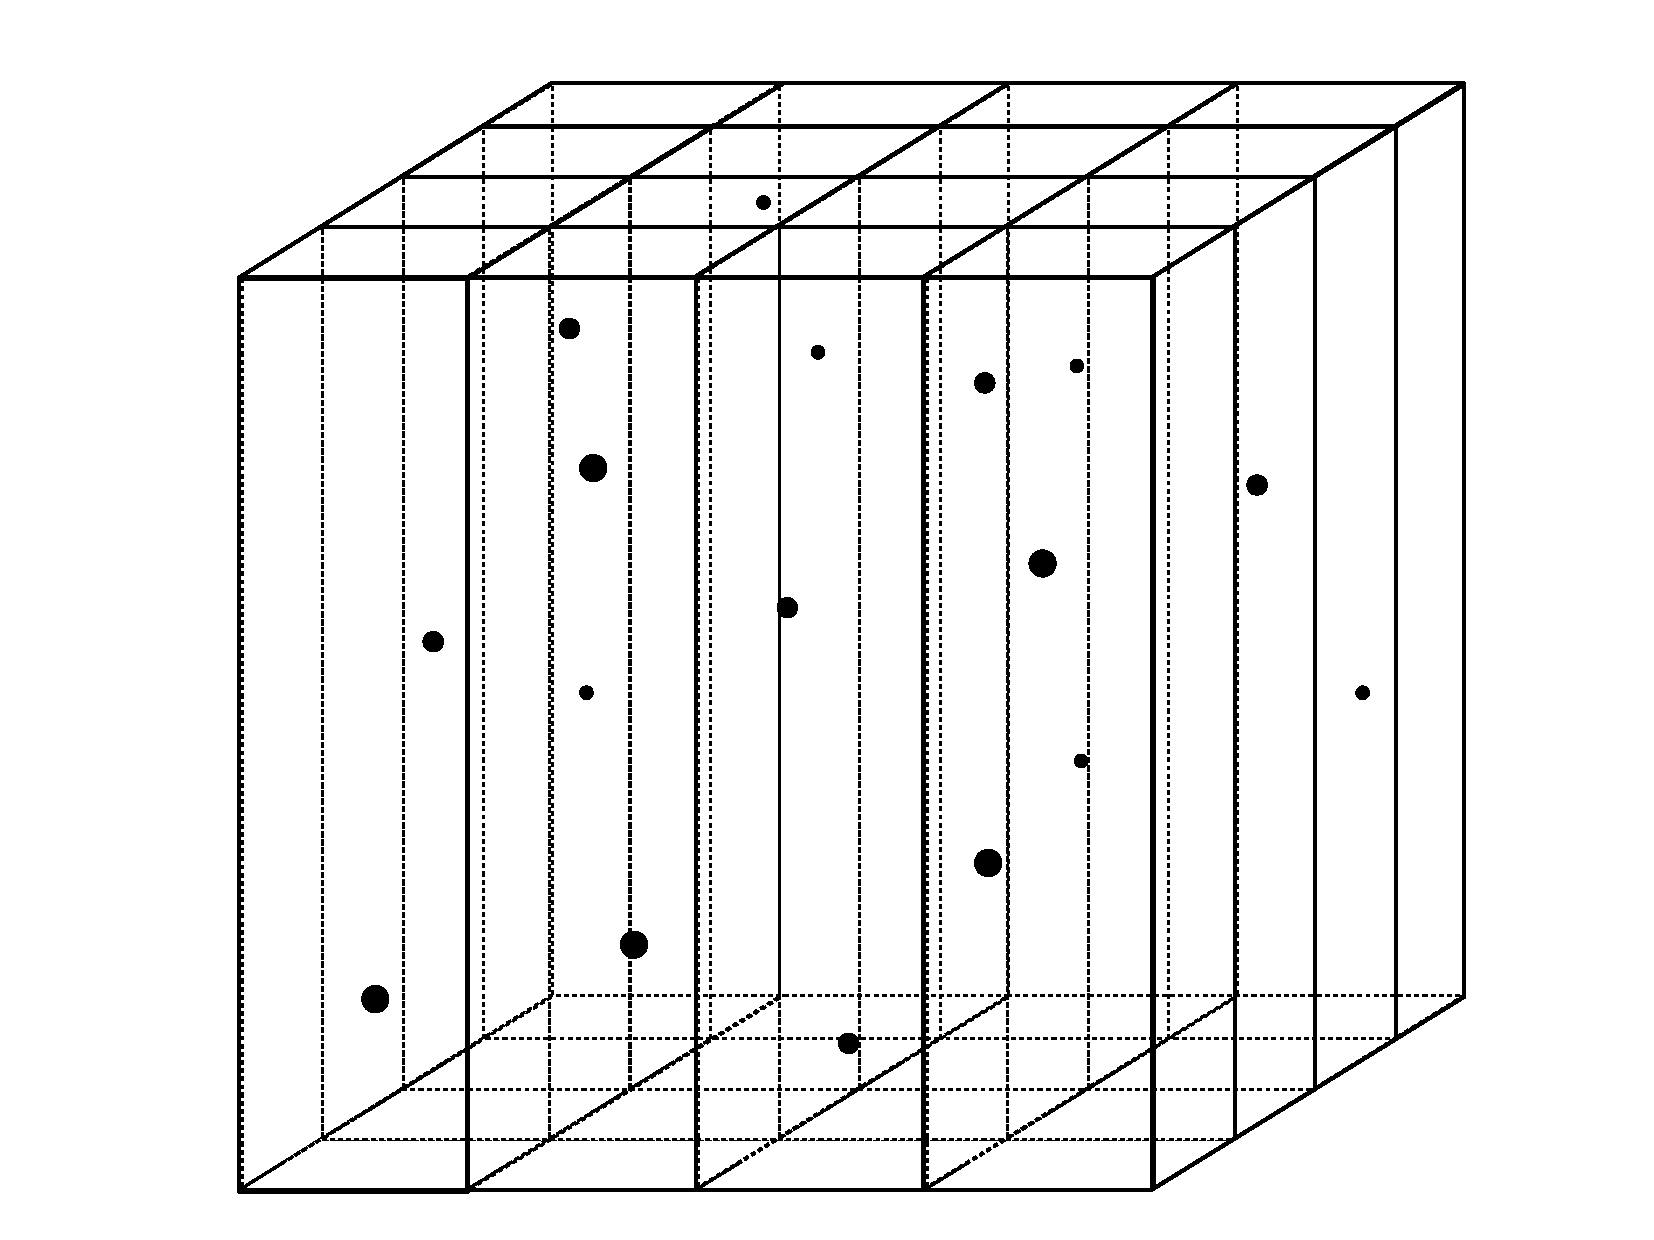
\includegraphics[width=10cm]{figures/1-04_2dd.pdf}
\caption{
Schematic representation of 2D domain decomposition.
This image corresponds to the actual decomposition of $64^{3}$ grid used for LES.
Entire domain is divided into $4 \times 4 = 16$ subdomains, each~with~$16 \times 16 \times 64$ nodes.
}
\label{fig:2dd}
\end{figure}



%%% =================== %%%
%%%      CHAPTER 2      %%%
%%% =================== %%%

% FIGURE 2-01 - TURBULENT FLOW ENERGY SPECTRA

\begin{figure}
\centering
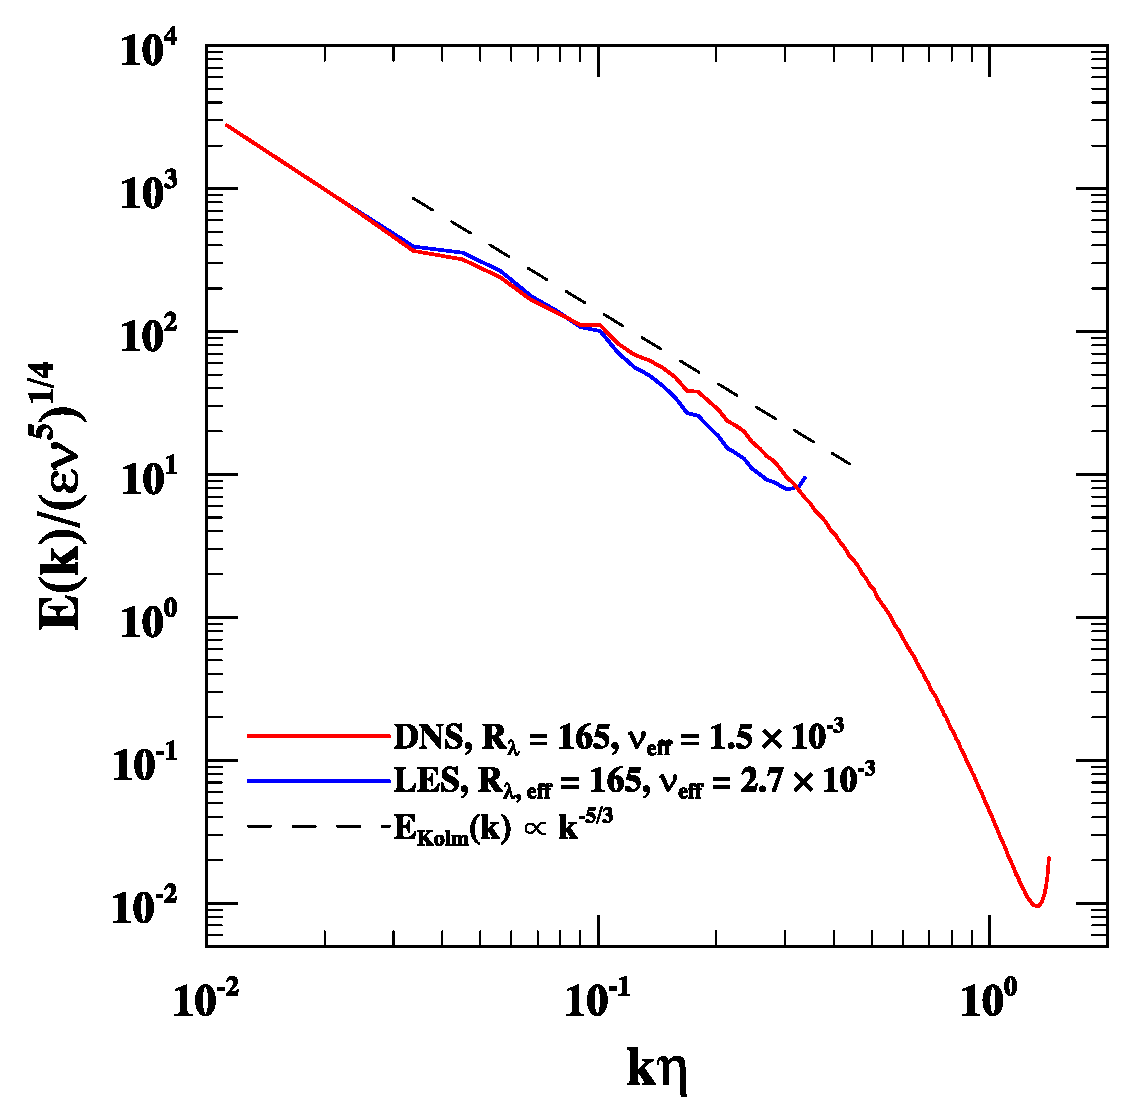
\includegraphics[width=8cm]{figures/2-01_spec.pdf}
\caption{
The normalised energy spectra of background turbulent flows for both DNS and LES.
Dashed line provides comparison with $k^{-5/3}$ curve of theoretical Kolmogorov spectrum (see Equation~\ref{eqn:kolm}) for inertial subrange.
}
\label{fig:spec}
\end{figure}
    
% FIGURE 2-02 - TURBULENT FLOW DISSIPATION SPECTRA

\begin{figure}
\centering
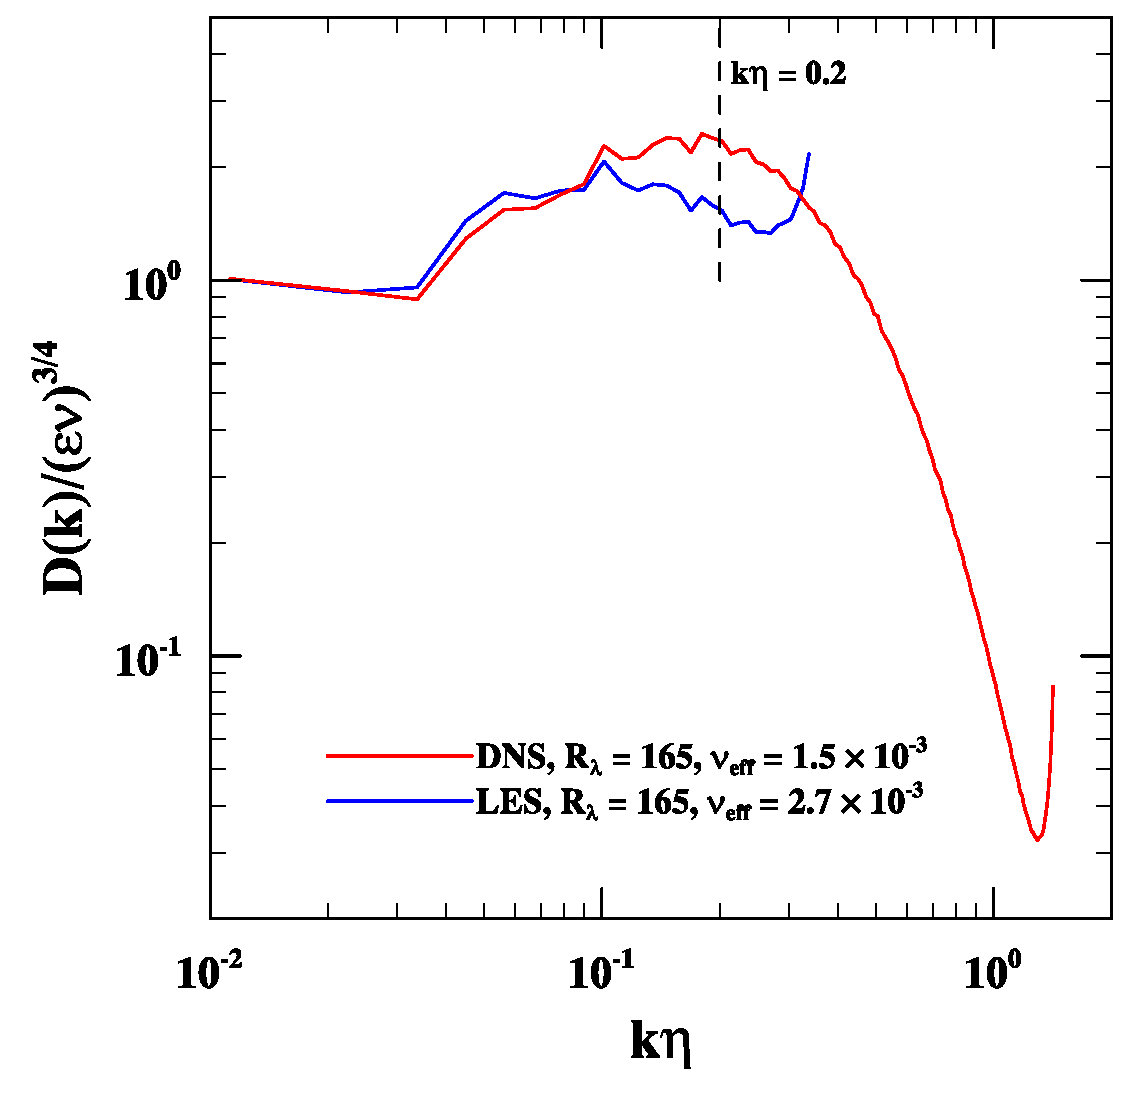
\includegraphics[width=8cm]{figures/2-02_diss.pdf}
\caption{
The normalised energy dissipation spectra of background turbulent flows for both DNS and LES.
Point where $D(k)$ is expected to be maximal (for $k \eta = 0.2$) is marked by dashed line. 
}
\label{fig:diss}
\end{figure}

% FIGURE 2-03 - ENERGY SPECTRA OF TURBULENT FLOWS MODULATED BY PARTICLES

\begin{figure}
\centering
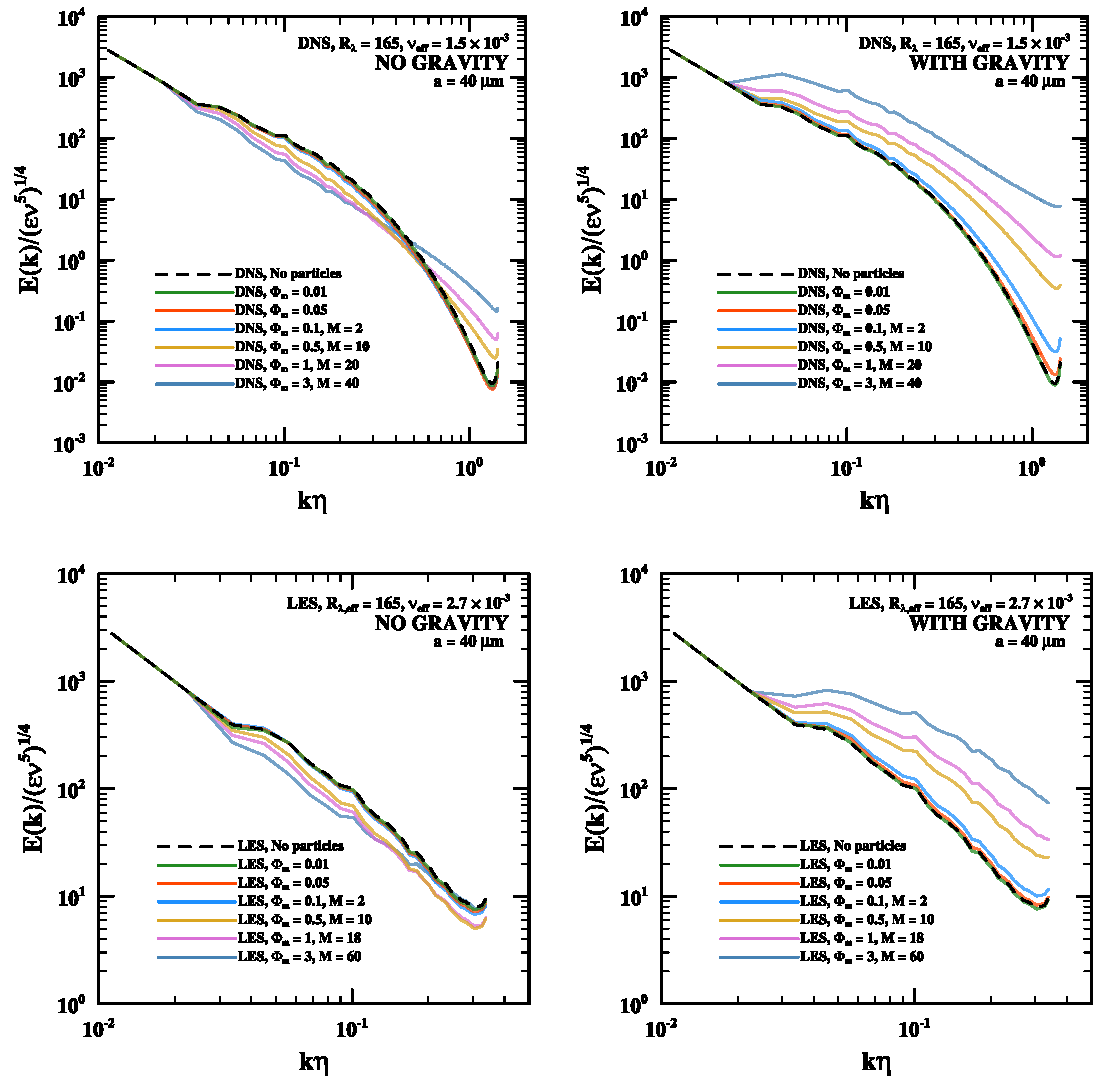
\includegraphics[width=13.5cm]{figures/2-03_modspec.pdf}
\caption{
The normalised energy spectra of turbulent flows with droplets of radii $40$~$\upmu\text{m}$, with and without gravity, as obtained using both DNS and LES with two-way momentum coupling and different particle mass loadings.
Dashed lines represent spectra without turbulence modulation by particles (see Figure \ref{fig:spec}).
For comparison (with DNS results only), see \textcite[Figure 4 therein]{Rosa2020}.
}
\label{fig:modspec}
\end{figure}

% FIGURE 2-04 - DISSIPATION SPECTRA OF TURBULENT FLOWS MODULATED BY PARTICLES
    
\begin{figure}
\centering
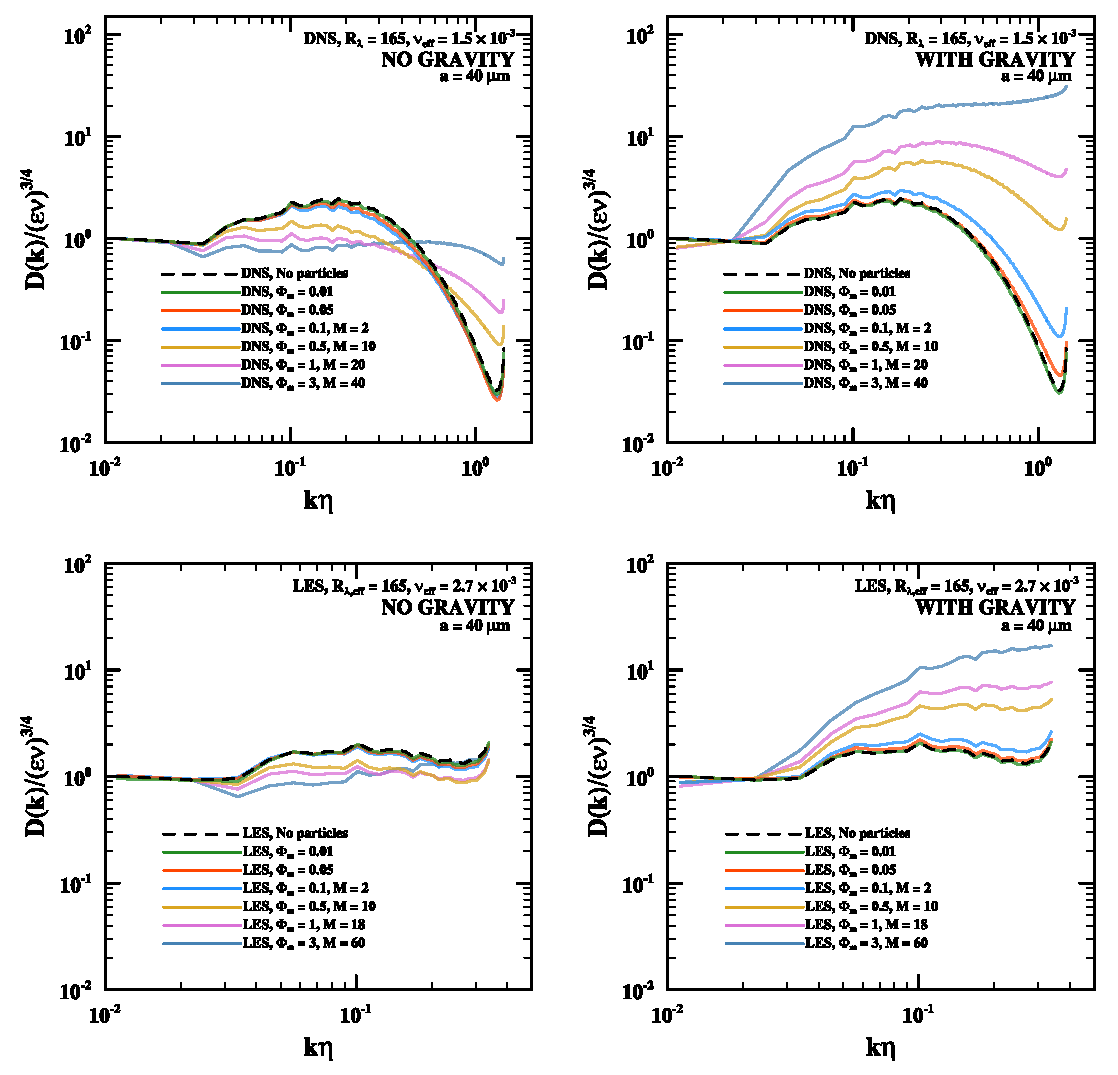
\includegraphics[width=13.5cm]{figures/2-04_moddiss.pdf}
\caption{
The normalised energy dissipation spectra of turbulent flows with droplets of radii $40$~$\upmu\text{m}$, with and without gravity, as obtained using both DNS and LES performed under two-way momentum coupling with different particle mass loadings.
Dashed lines represent dissipation spectra without turbulence modulation by particles (see Figure \ref{fig:diss}).
For comparison (DNS only), see Figure 5 in \textcite{Rosa2020}.
}
\label{fig:moddiss}
\end{figure}

% FIGURE 2-05 - PARAMETERS OF TURBULENT FLOWS MODULATED BY PARTICLES

\begin{figure}
\centering
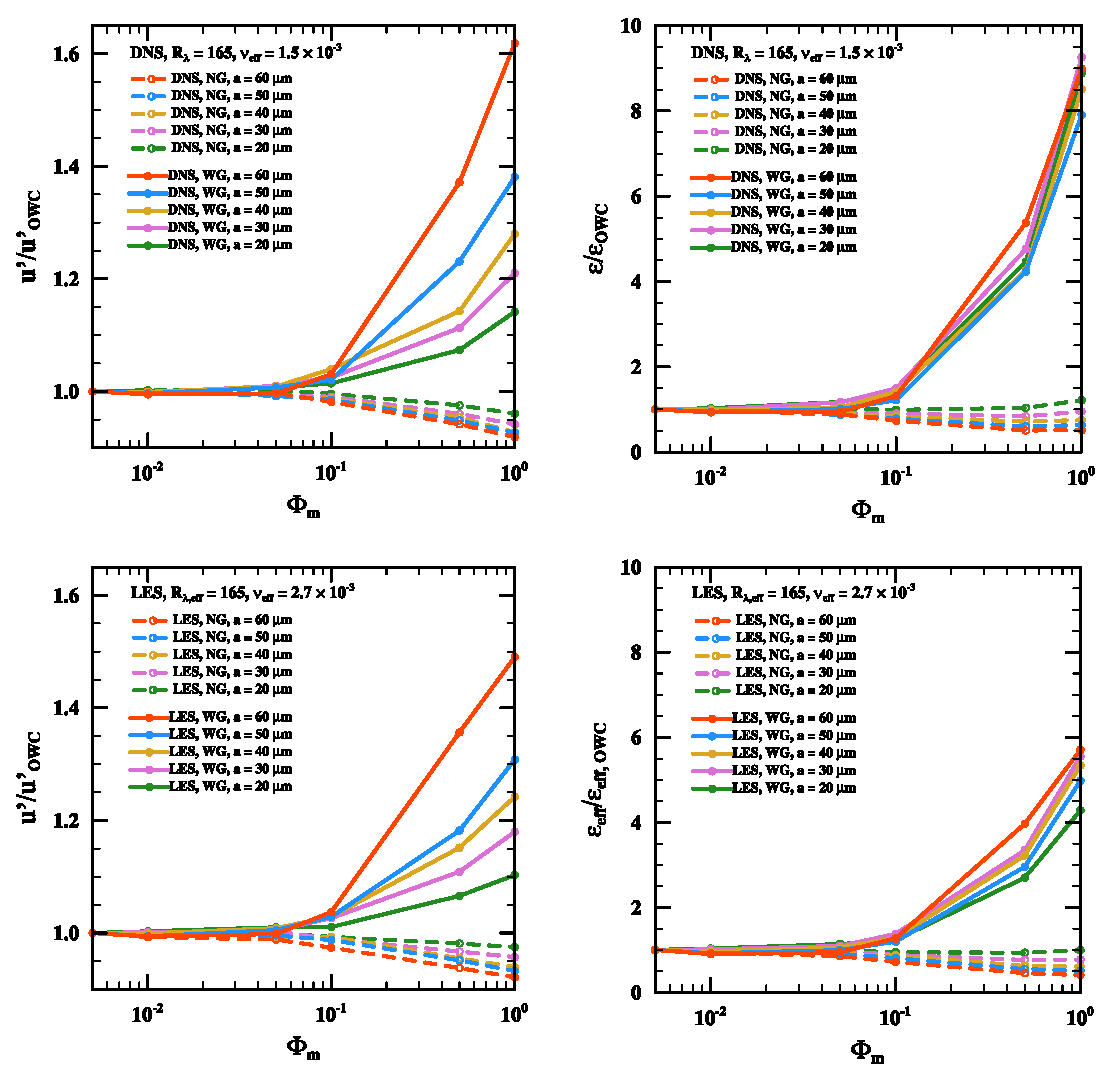
\includegraphics[width=13.5cm]{figures/2-05_modstat.pdf}
\caption{
Time averaged statistics of turbulent flows as obtained by DNS and LES under two-way momentum coupling, normalised by the corresponding statistics from simulations without turbulence modulation (OWC).
Plotted statistics include: the effective energy dissipation rate, $\epsilon_{\text{eff}}$ (top figures for DNS and LES, respectively), and the RMS fluctuating velocity, $u'$ (bottom figures, likewise).
WG denotes simulations with gravity (continuous lines); NG -- without gravity (dashed lines).
For comparison (DNS only), see Figure 11 in \textcite{Rosa2020}.
}
\label{fig:modstat}
\end{figure}

% FIGURE 2-06 - RDF AND RRV FOR OWC SIMULATIONS

\begin{figure}
\centering
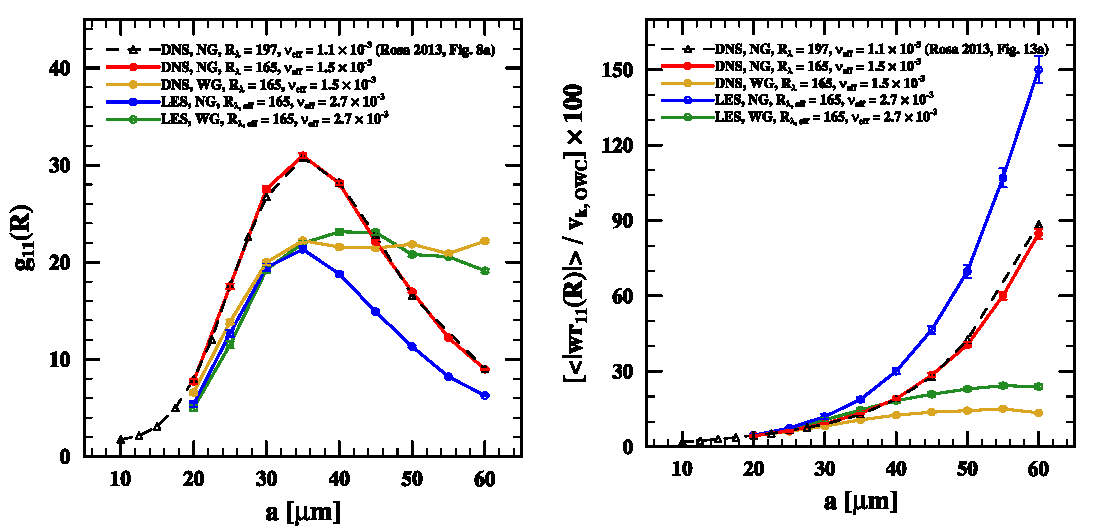
\includegraphics[width=13.5cm]{figures/2-06_owcrdfrrv.pdf}
\caption{
The values of the radial distribution function (RDF, left) and the radial relative velocity (RRV, right) at contact distance for simulations under one-way momentum coupling.
Results include data from both DNS and LES simulations, with (WG) and without (NG) gravity.
}
\label{fig:owcrdfrrv}
\end{figure}

% FIGURE 2-07 - COLLISON KERNELS FOR OWC SIMULATIONS

\begin{figure}[h]
\centering
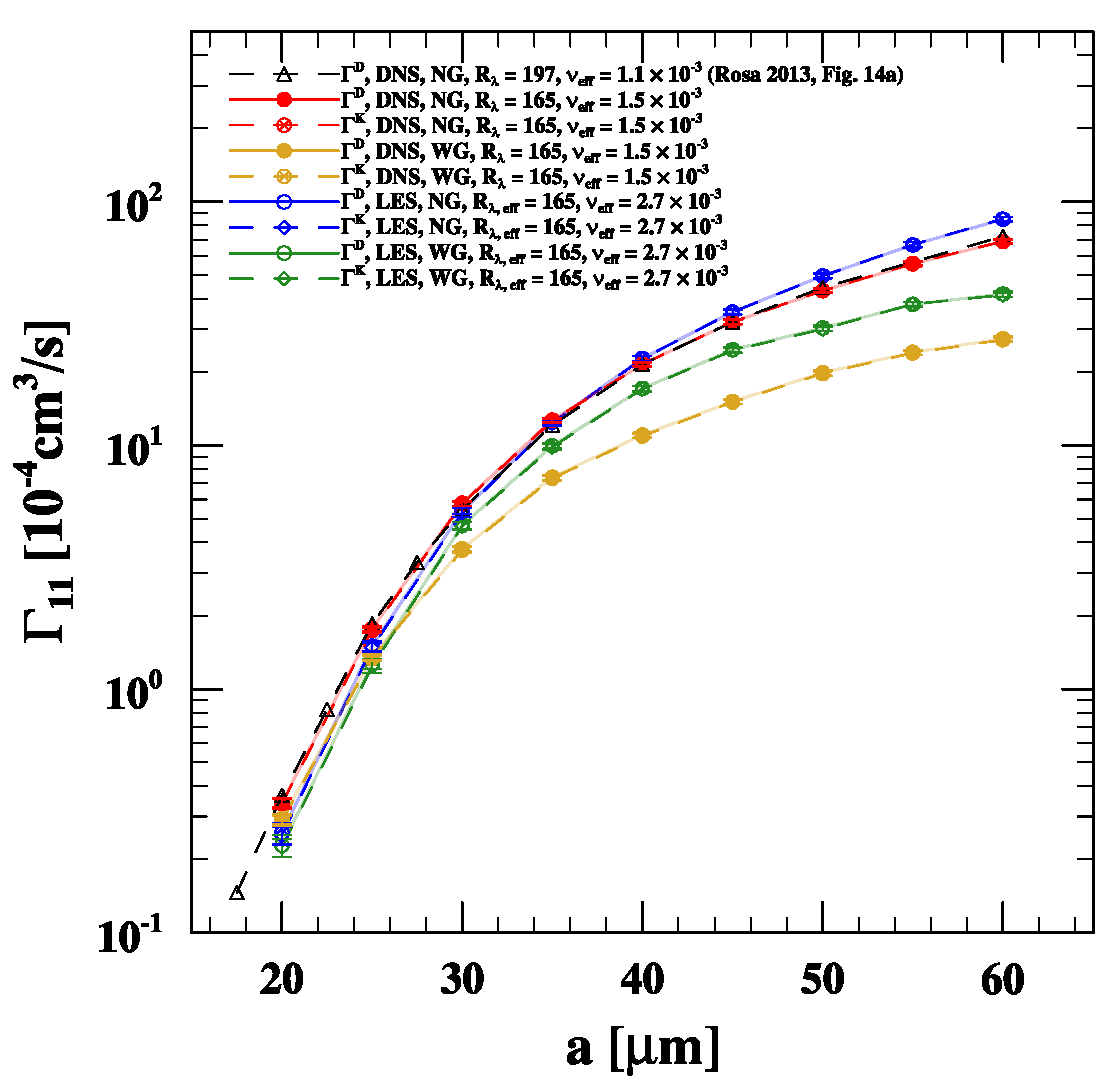
\includegraphics[width=10cm]{figures/2-07_owcgamma.pdf}
\caption{
The values of both dynamic and kinematic collision kernels for simulations under one-way momentum coupling.
Results include data from both DNS and LES simulations, with (WG) and without (NG) gravity.
Continuous lines represent values for dynamic kernel ($\Gamma_{11}^D$) and dashed ones (almost overlaid on continuous ones due to their close agreement) -- for kinematic kernel ($\Gamma_{11}^K$). 
}
\label{fig:owcgamma}
\end{figure}

% FIGURE 2-08 - RDF FOR TWC SIMULATIONS

\begin{figure}
\centering
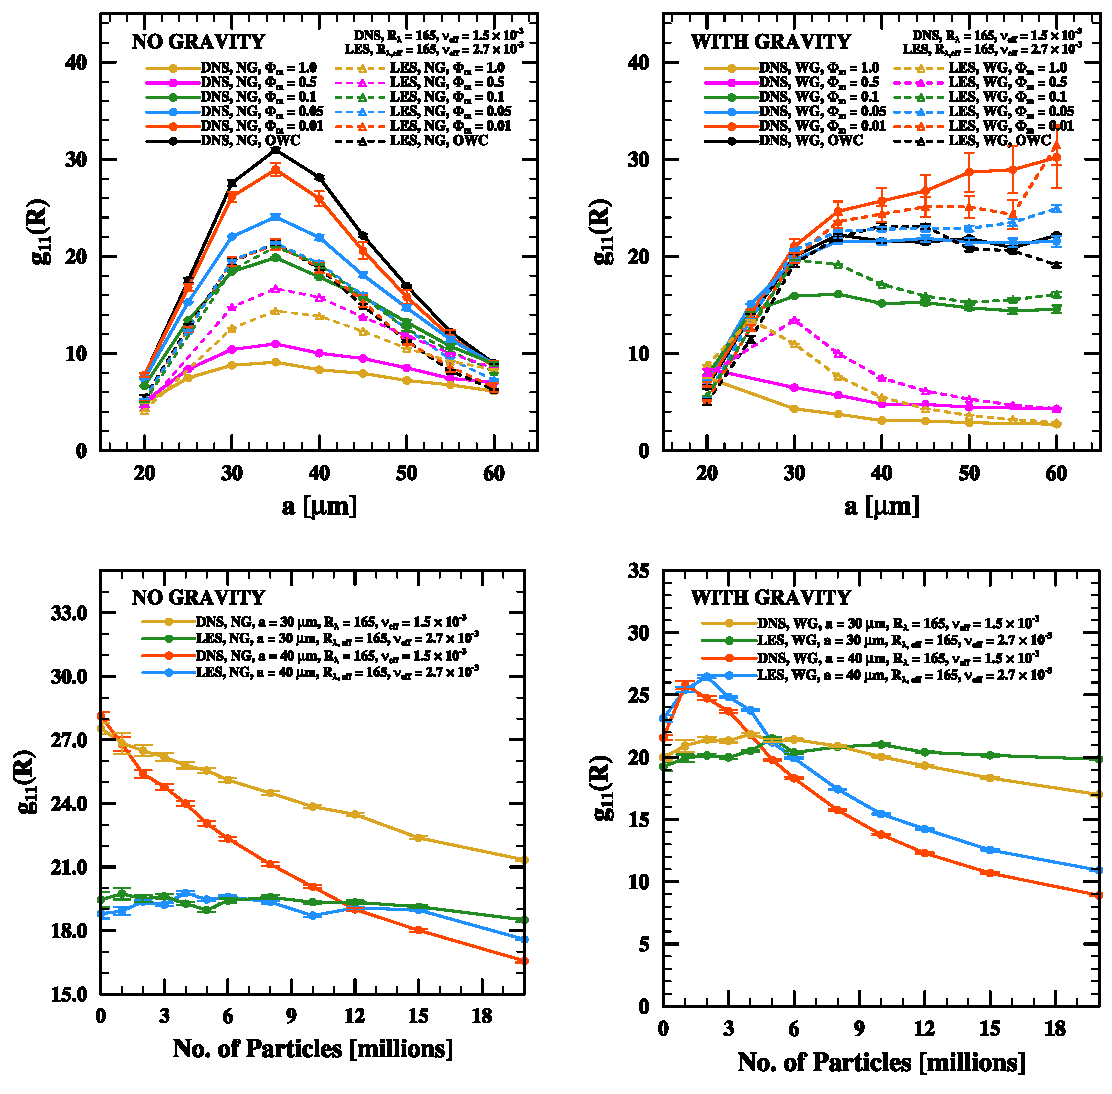
\includegraphics[width=13.5cm]{figuress/2-08_twcrdf.pdf}
\caption{
The values of radial distribution function (RDF) at contact distance for simulations under two-way momentum coupling using both DNS and LES.
Top plots show relation of RDF on particle radius for several fixed values of mass loading, $\Phi_m$ (also compared with results for OWC).
Bottom ones show the dependence of RDF on the number of particles (in millions) for particles with radii $30$~$\upmu\text{m}$ and $40$~$\upmu\text{m}$.
Plots on the left show results without effects of gravity (NG), and those on the right consider settling particles (WG).
}
\label{fig:twcrdf}
\end{figure}

% FIGURE 2-09 - RDF FOR TWC SIMULATIONS WITH LARGER MASS LOADINGS

\begin{figure}
\centering
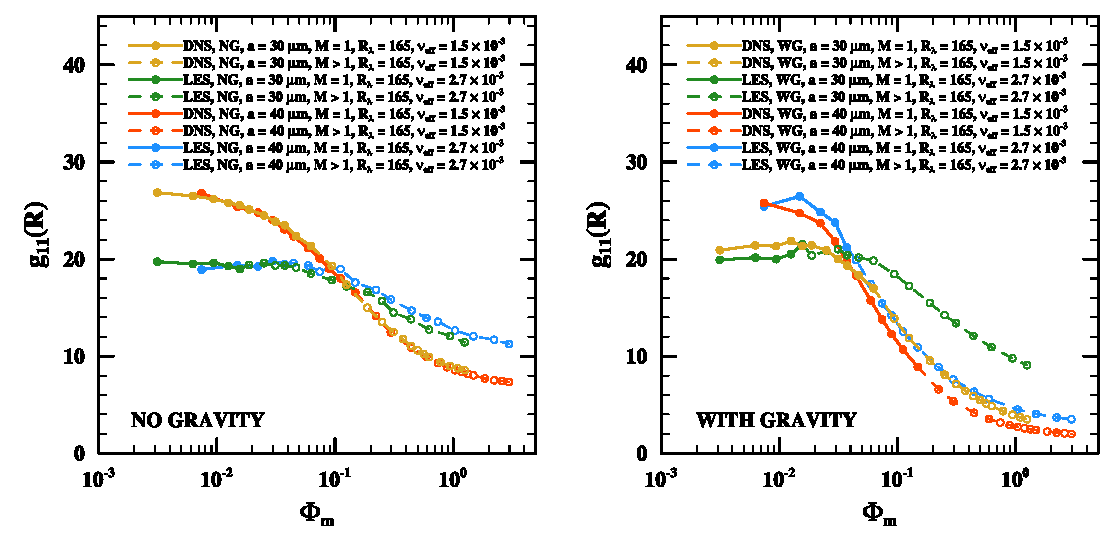
\includegraphics[width=13.5cm]{figures/2-09_twcrdfext.pdf}
\caption{
The values of RDF for wider range of mass loadings.
It may be considered as an extension of bottom plots from Figure \ref{fig:twcrdf} where scope was limited to $20$ million particles (${\Phi_m \approx 0.1}$).
Here, results include wider range of mass loadings where TWC should be most prominent (i.e. around $0.1$ to $1$) and where it may even not be sufficient (i.e. four-way coupling regime for $\Phi_m > 1$).
Continuous lines represent simulations without super-particle parameterisation ($M=1$), while dashed ones show where super-particle parameterisation was necessary to obtain larger mass loadings.
For precise information on values of $M$ for each simulation, see Appendix \ref{app:spp}. 
}
\label{fig:twcrdfext}
\end{figure}

% FIGURE 2-10 - RRV FOR TWC SIMULATIONS

\begin{figure}
\centering
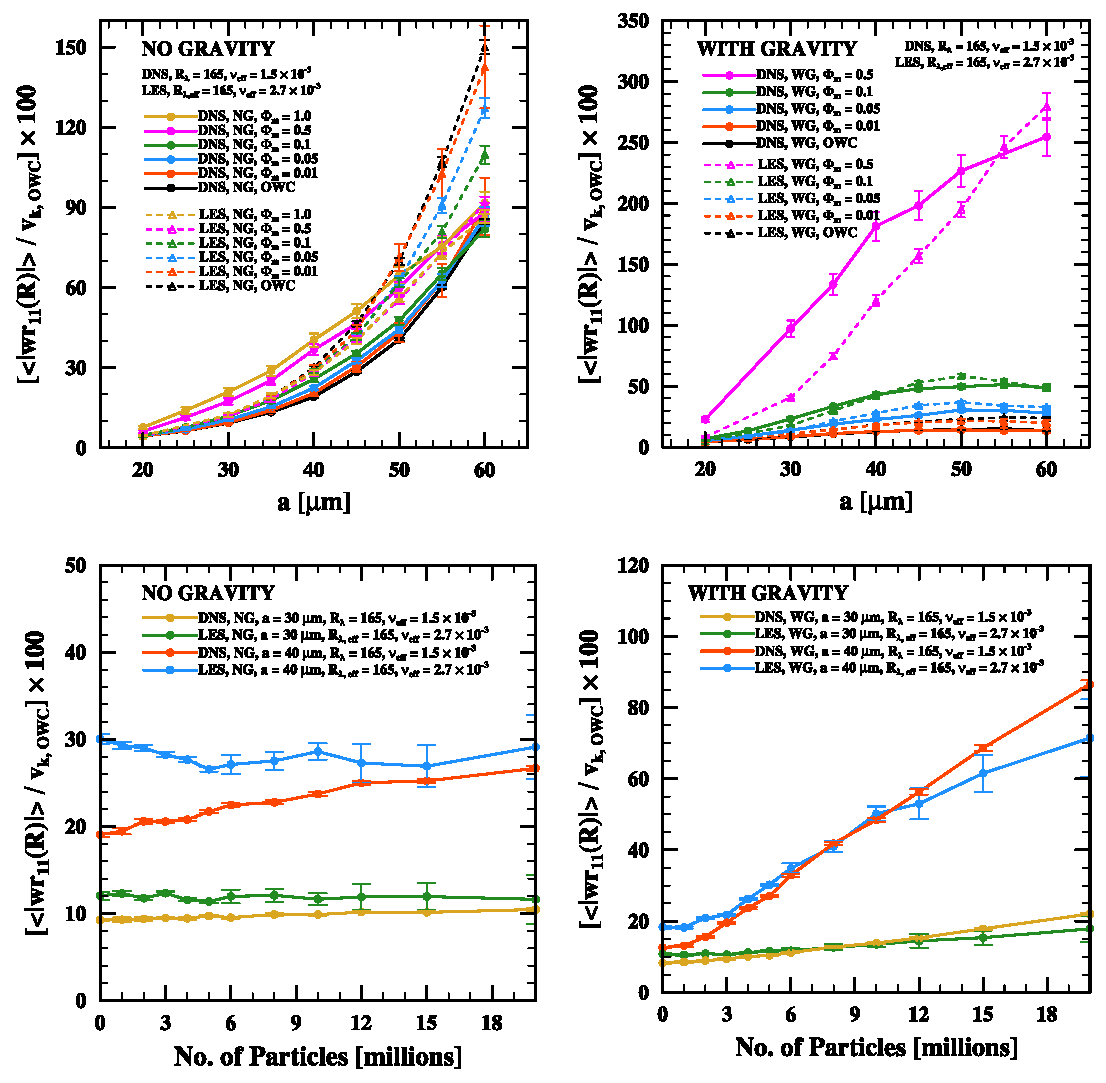
\includegraphics[width=13.5cm]{figures/2-10_twcrrv.pdf}
\caption{
The values of radial relative velocity (RRV) at contact distance for simulations under two-way momentum coupling using both DNS and LES.
Consistent with Figure \ref{fig:twcrdf}.
}
\label{fig:twcrrv}
\end{figure}

% FIGURE 2-11 - RRV FOR TWC SIMULATIONS WITH LARGER MASS LOADINGS

\begin{figure}
\centering
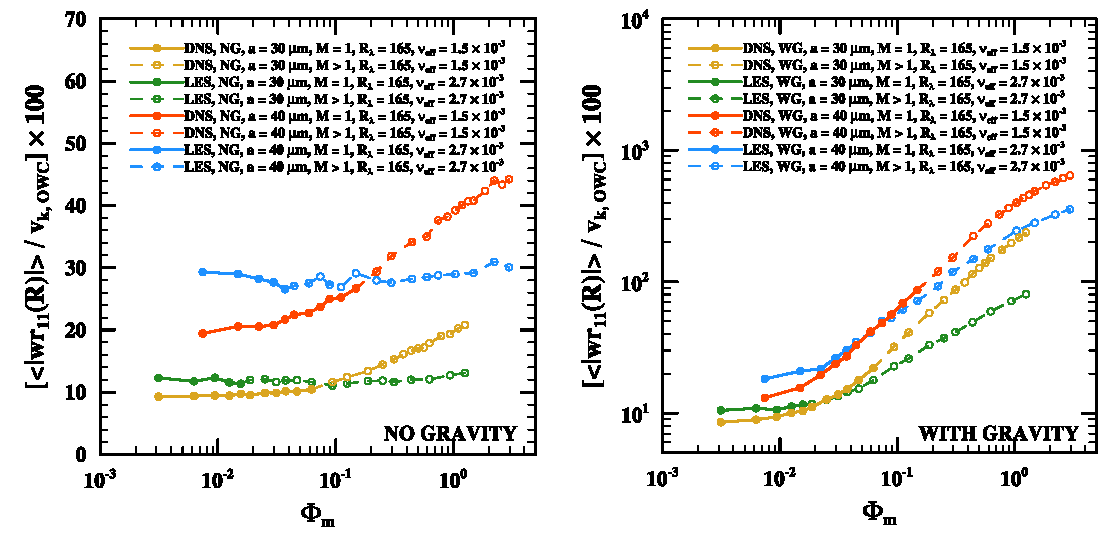
\includegraphics[width=13.5cm]{figures/2-11_twcrrvext.pdf}
\caption{
The values of RRV for wider range of mass loadings.
Consistent with Figure \ref{fig:twcrdfext}.
}
\label{fig:twcrrvext}
\end{figure}

% FIGURE 2-12 - DYNAMIC COLLISION KERNELS FOR TWC SIMULATIONS

\begin{figure}
\centering
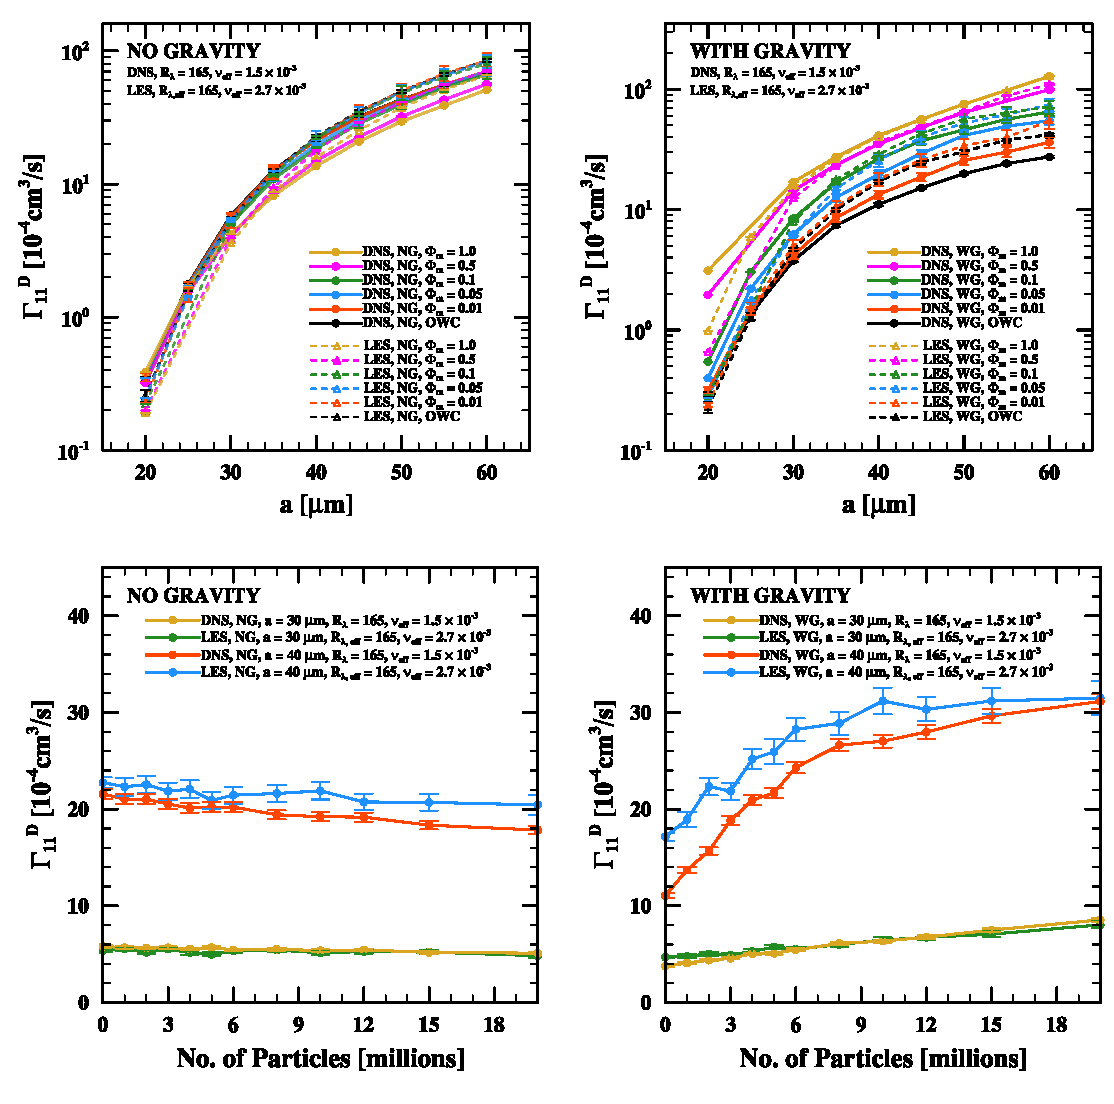
\includegraphics[width=13.5cm]{figures/2-12_twcgamma.pdf}
\caption{
The values of dynamic collision kernel ($\Gamma_{11}^D$) for simulations under two-way momentum coupling using both DNS and LES.
Consistent with Figure \ref{fig:twcrdf}.
}
\label{fig:twcgamma}
\end{figure}

% FIGURE 2-13 - DYNAMIC COLLISION KERNELS FOR SIMULATIONS WITH LARGER MASS LOADINGS

\begin{figure}
\centering
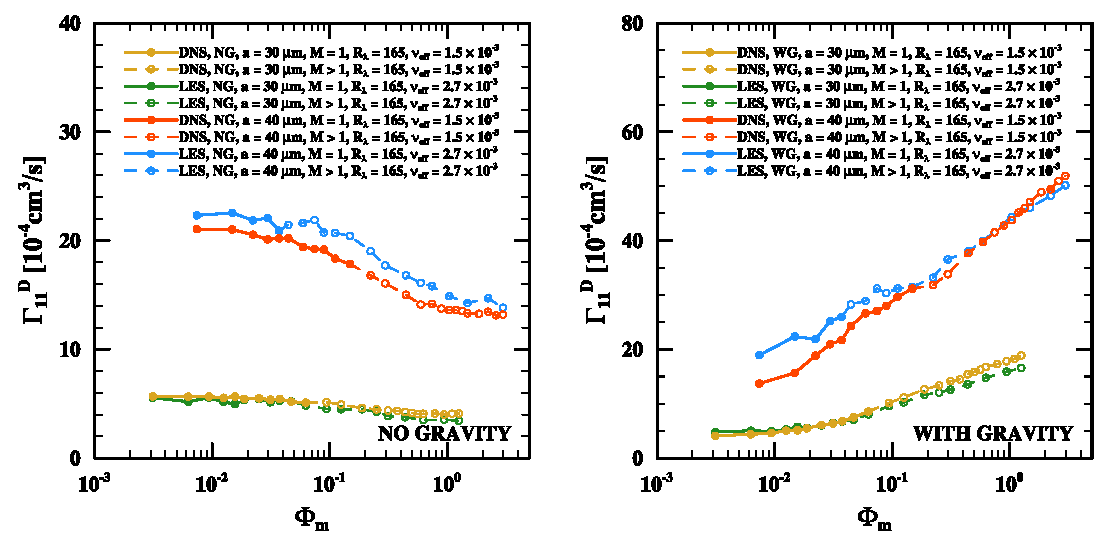
\includegraphics[width=13.5cm]{figures/2-13_twcgammaext.pdf}
\caption{
The values of dynamic collision kernel for wider range of mass loadings.
Consistent with Figure \ref{fig:twcrdfext}.
}
\label{fig:twcgammaext}
\end{figure}



%%% =================== %%%
%%%      CHAPTER 3      %%%
%%% =================== %%%

% FIGURE 3-01 - HALO REGIONS

\begin{figure}
\centering
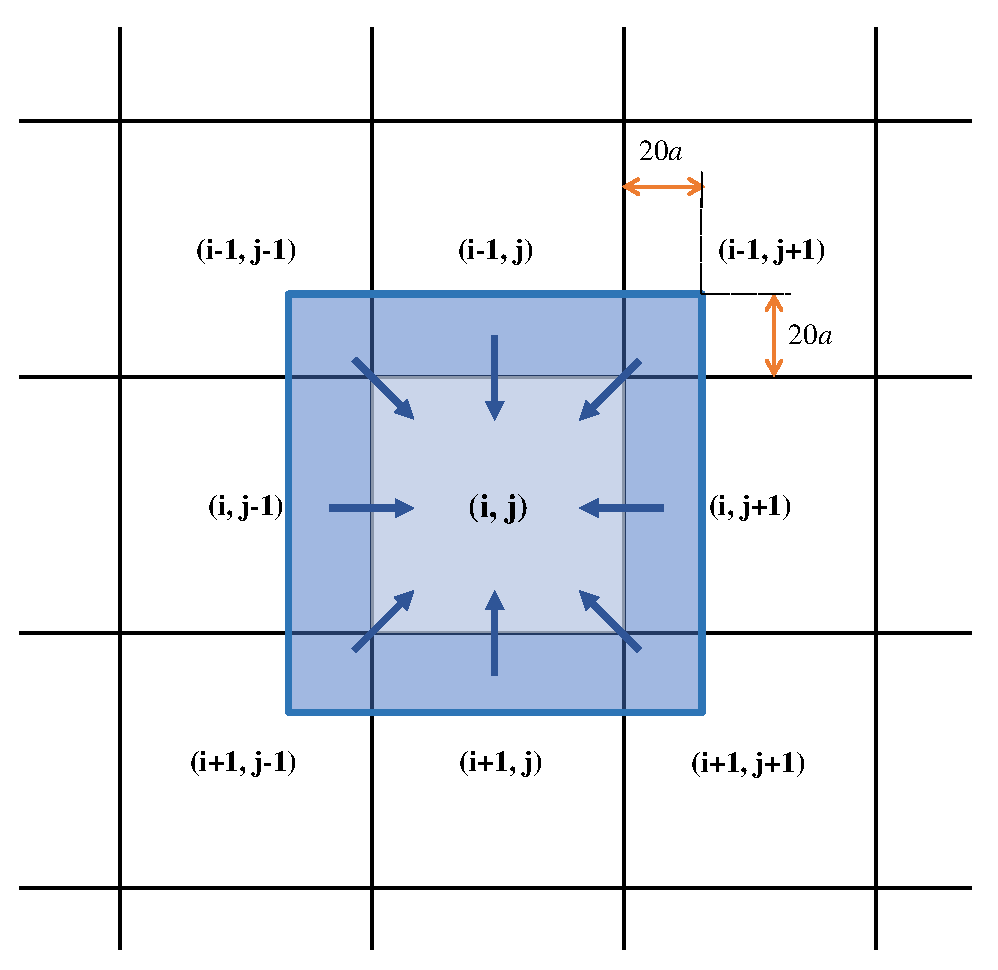
\includegraphics[width=9cm]{figures/3-01_halo.pdf}
\caption{
The halo region of the host process that overlaps with eight neighbouring subdomains in 2D decomposition.
The range of overlap is $10R = 20a$, which is the largest possible outer radius of spherical shells used to calculate kinematic statistics of particles for particle located at the subdomain boundary.
Arrows indicate the direction of data transfer.
Illustration based on Figure 3 in \textcite{Ayala2014}. 
}
\label{fig:halo}
\end{figure}

% FIGURE 3-02 - SIMPLE TIMINGS FOR OWC SIMULATIONS

\begin{figure}
\centering
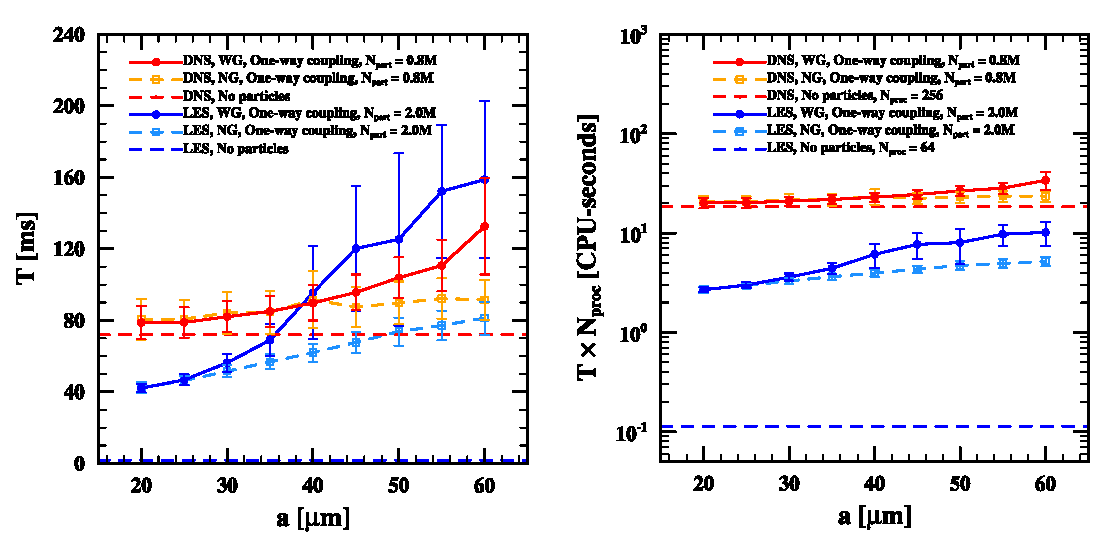
\includegraphics[width=13.5cm]{figures/3-02_pfsowc.pdf}
\caption{
Time-averaged wall-clock times per step by itself (left) and multiplied by number of parallel processes used to execute code (right, in log scale) for simulations under one-way momentum coupling (OWC) presented as a function of particle radii.
Both results for DNS and LES are presented, with (WG) and without (NG) gravity.
Horizontal dashed lines represent values for simulations without particles.
}
\label{fig:pfsowc}
\end{figure}

% FIGURE 3-03 - SIMPLE TIMINGS FOR TWC SIMULATIONS

\begin{figure}
\centering
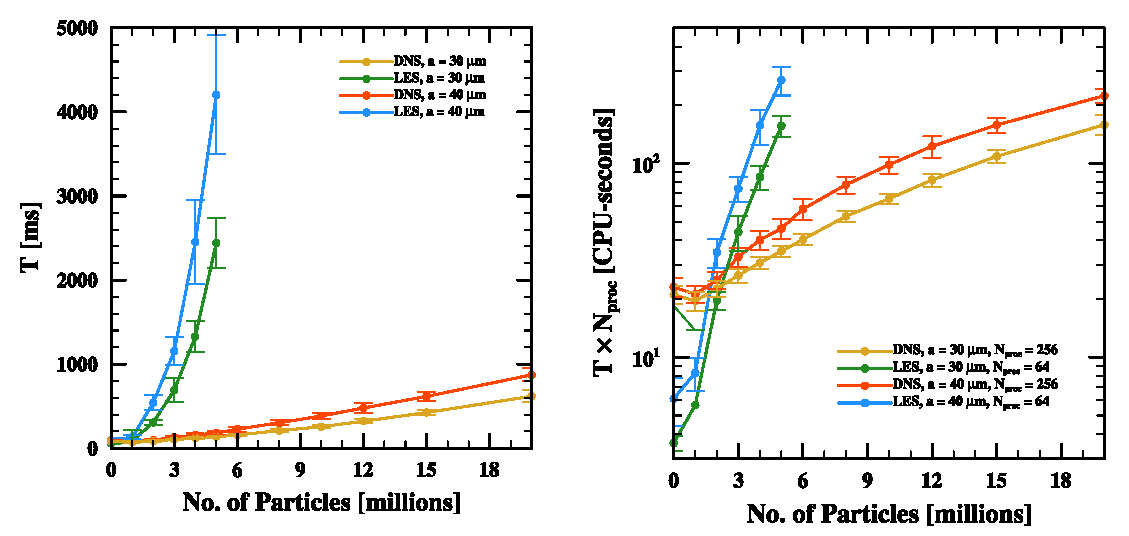
\includegraphics[width=13.5cm]{figures/3-03_pfstwc.pdf}
\caption{
Time-averaged wall-clock times per step by itself (left) and multiplied by number of parallel processes used to execute code (right, in log scale) for simulations under two-way momentum coupling (TWC, with gravity)as a function of  the number of computational particles. 
Results for both DNS and LES are presented.
}
\label{fig:pfstwc}
\end{figure}
    
% FIGURE 3-04 - SIMPLE TIMINGS FOR DNS FOR DIFFERENT CPU NODE COUNT

\begin{figure}
\centering
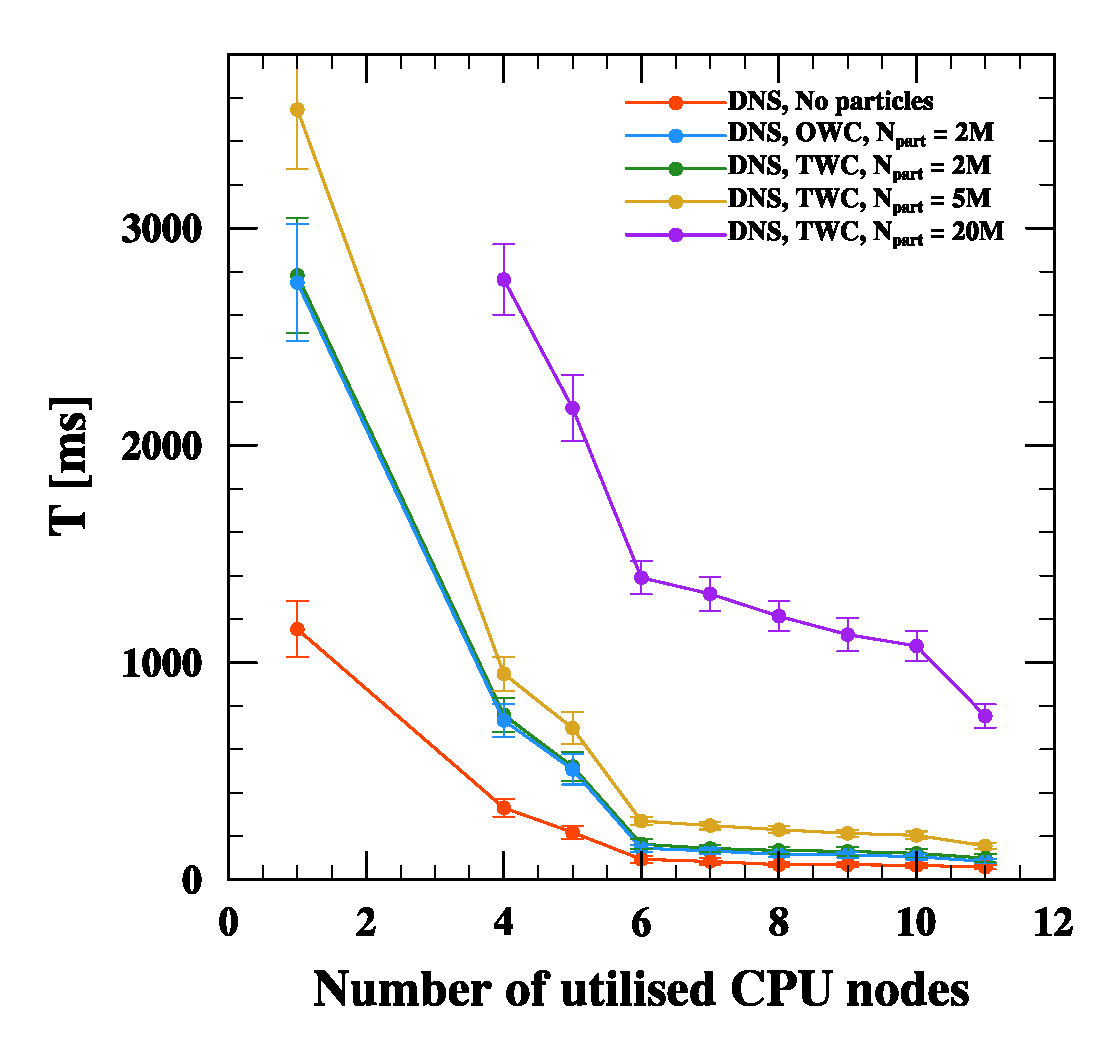
\includegraphics[width=8cm]{figures/3-04_pfspfn.pdf}
\caption{
Time-averaged wall-clock times per step for DNS, depending on the limited number of computational nodes on \emph{Okeanos} supercomputer (24 CPU cores per node).
DNS supports up to $256$ parallel processes in execution, hence value of $11$ represents optimal saturation of processes with available CPU cores.
}
\label{fig:pfspfn}
\end{figure}

% FIGURE 3-05 - SIMPLE TIMINGS FOR TWC RELATED TO RDF

\begin{figure}
\centering
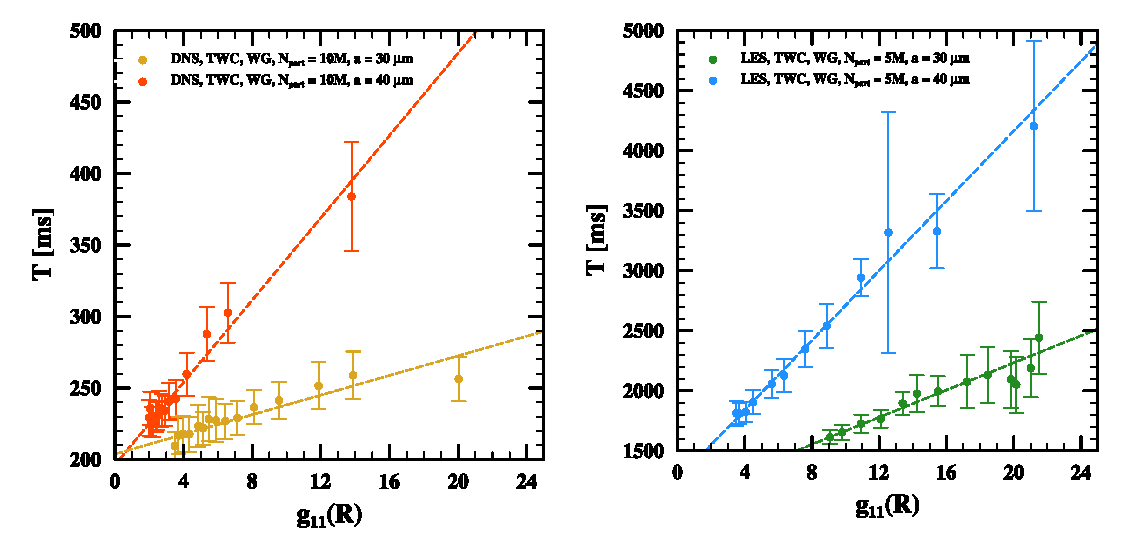
\includegraphics[width=13.5cm]{figures/3-05_pfsrdf.pdf}
\caption{
Time-averaged wall-clock times per step for DNS (left) and LES (right) simulations under two-way momentum coupling (TWC) with fixed number of computational particles (10 million for DNS, 5 million for LES) and radii ($30$~$\upmu\text{m}$ and $40$~$\upmu\text{m}$), depending on the estimated values of the radial distribution function at contact range (RDF at $r=R$).
Dashed lines represent linear fit of included results weighted by the inverse variance of respective data points.
}
\label{fig:pfsrdf}
\end{figure}

% FIGURE 3-06 - PROFILE DATA FOR OWC LES

\begin{figure}
\centering
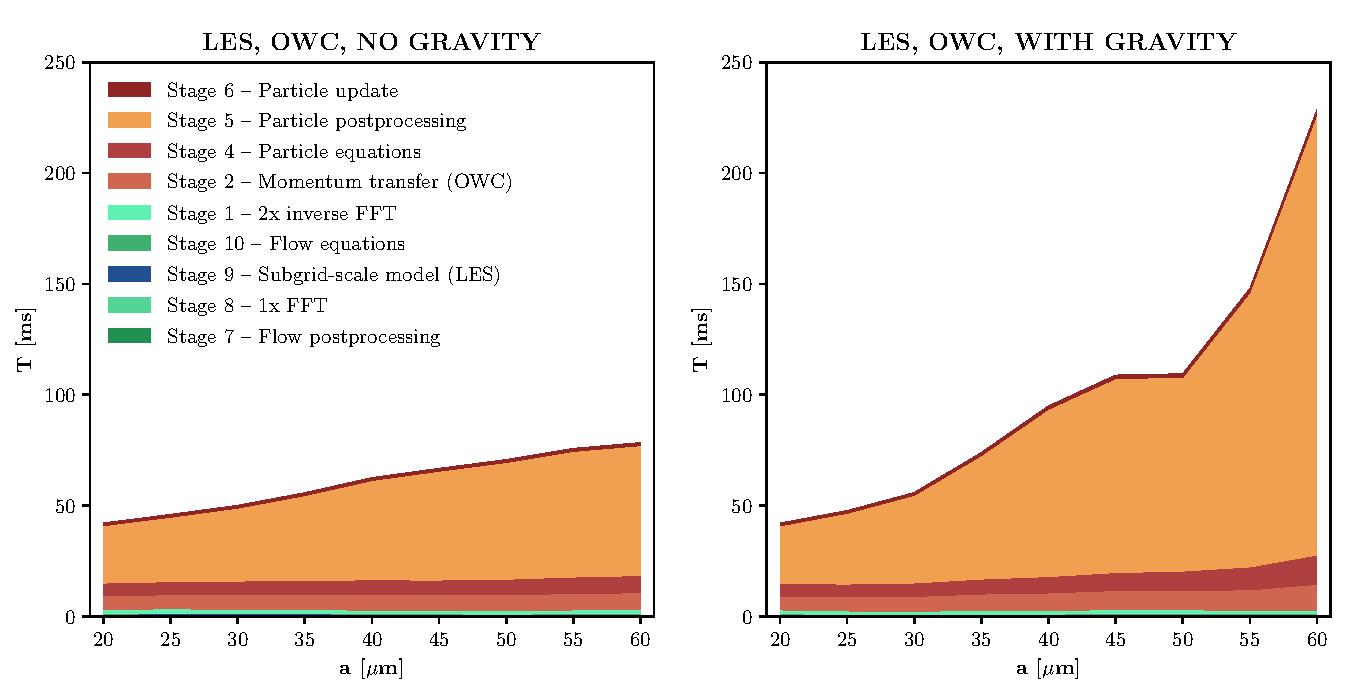
\includegraphics[width=13.5cm]{figures/3-06_pffowcles.pdf}
\caption{
Performance profile for OWC LES simulations with and without gravity (right and left, respectively).
Layers of different colours represent average wall-clock time per step for given stage ($T_i$) and are ordered as they appear in code.
For clarity, all stages related to the fluid flow computations are grouped together and represented by the bottom layers.
}
\label{fig:pffowcles}
\end{figure}

% FIGURE 3-07 - FLUID AND PARTICLE PROCESSING TIMES FOR OWC LES

\begin{figure}
\centering
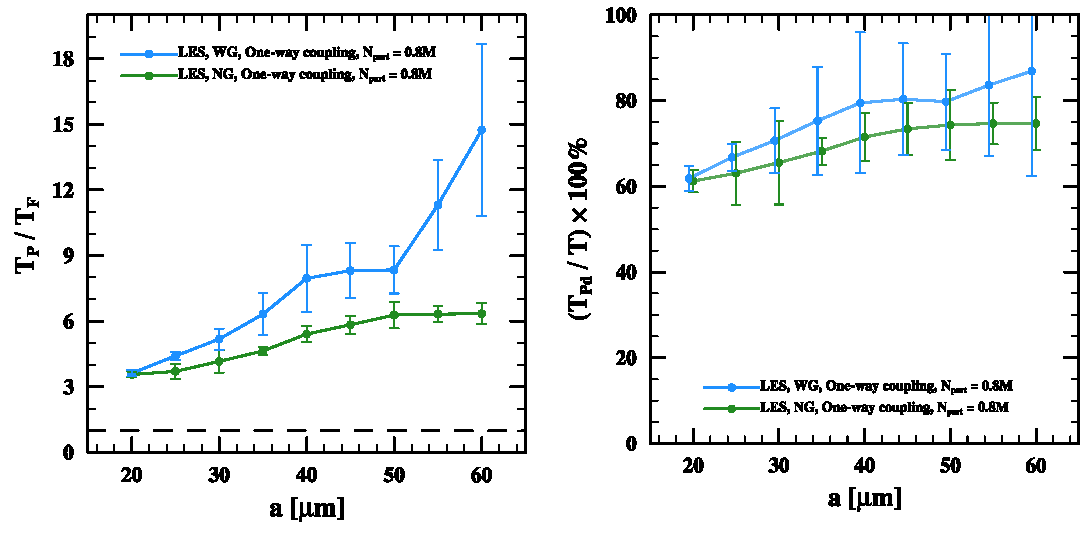
\includegraphics[width=13.5cm]{figures/3-07_pffowclesex.pdf}
\caption{
The ratio of average wall-clock times spent on processing particles, $T_{\text{P}}$, and the fluid flow, $T_{\text{F}}$ (left); and average percentage of overall wall-clock time per step occupied by particle postprocessing tasks, $(T_{\text{Pd}} / T)$ (right).
Both statistics are shown for for OWC LES with and without gravity.
Plots on the right have slight horizontal offset added to make uncertainty bars more visible.
}
\label{fig:pffowclesex}
\end{figure}

% FIGURE 3-08 - PROFILE DATA FOR TWC LES

\begin{figure}
\centering
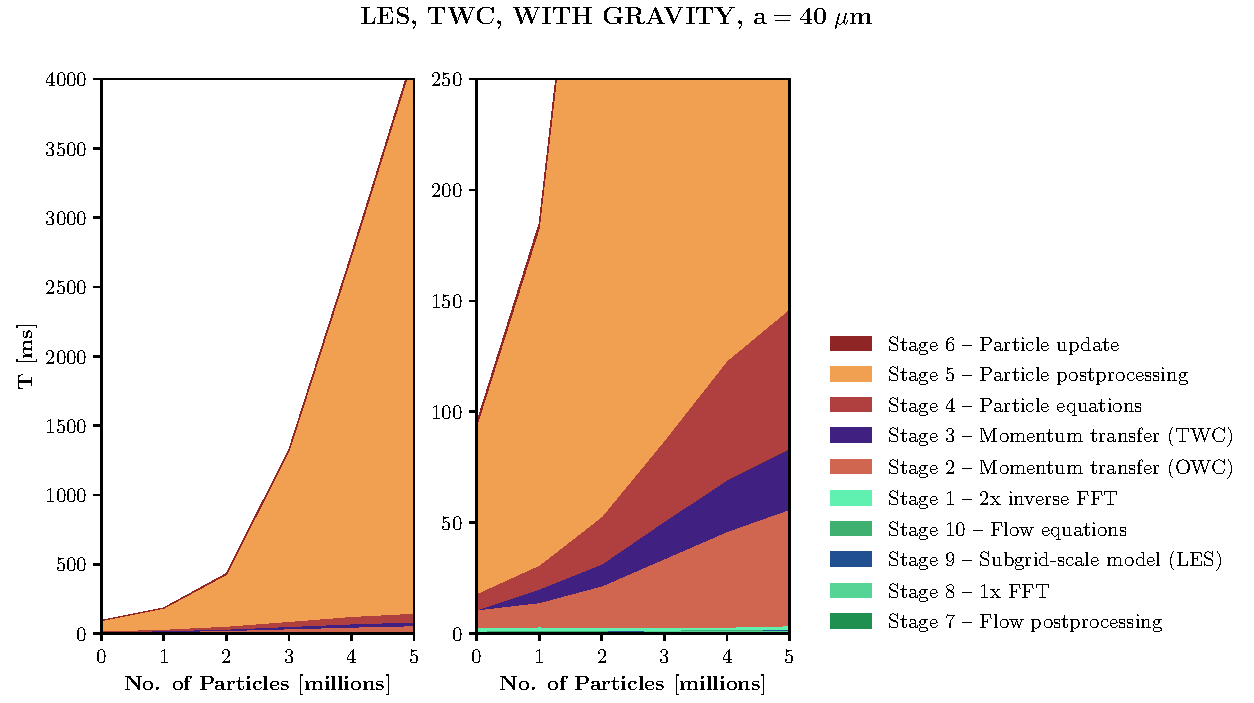
\includegraphics[width=13.5cm]{figures/3-08_pfftwcles.pdf}
\caption{
Performance profile for TWC LES simulations with gravity for droplets with $40$~$\upmu\text{m}$ radius.
Consistent with Figure \ref{fig:pffowcles}.
Both plots present profiles for the same range of simulations but the one on the right focuses on smaller span of values on the $y$-axis to ``magnify'' data pertaining to timings other than $T_5$ ($ = T_{\text{Pd}}$) that dominates plot on the left.
The leftmost profile (for $0$ on $x$-axis) was provided for corresponding OWC simulation with $N_{\text{part}} = 800\text{k}$. 
}
\label{fig:pfftwcles}
\end{figure}

% FIGURE 3-09 - PROFILE DATA FOR TWC DNS

\begin{figure}
\centering
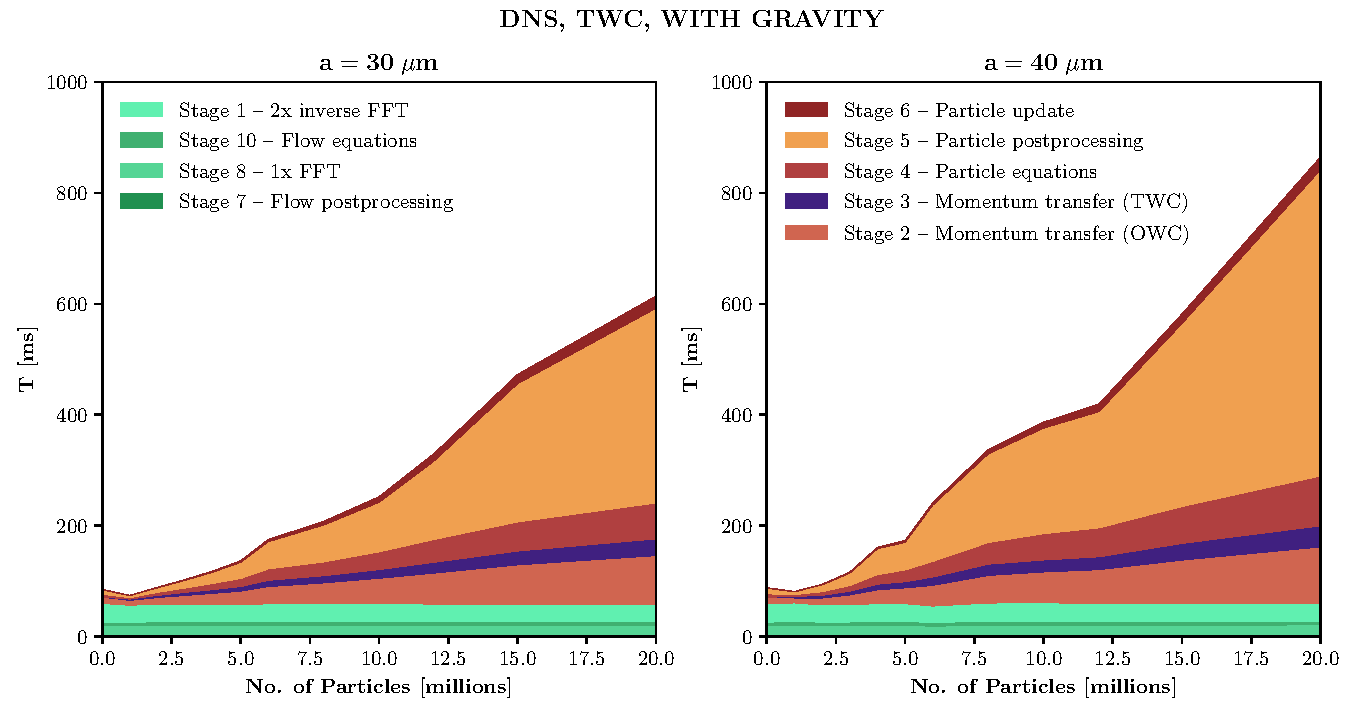
\includegraphics[width=13.5cm]{figures/3-09_pfftwcdns.pdf}
\caption{
Performance profile for TWC DNS simulations with gravity for droplets with radii $30$~$\upmu\text{m}$ (left) and $40$~$\upmu\text{m}$ (right).
Consistent with Figures \ref{fig:pffowcles} and \ref{fig:pfftwcles}.
}
\label{fig:pfftwcdns}
\end{figure}

% FIGURE 3-10 - FLUID AND PARTICLE PROCESSING TIMES FOR TWC WG

\begin{figure}
\centering
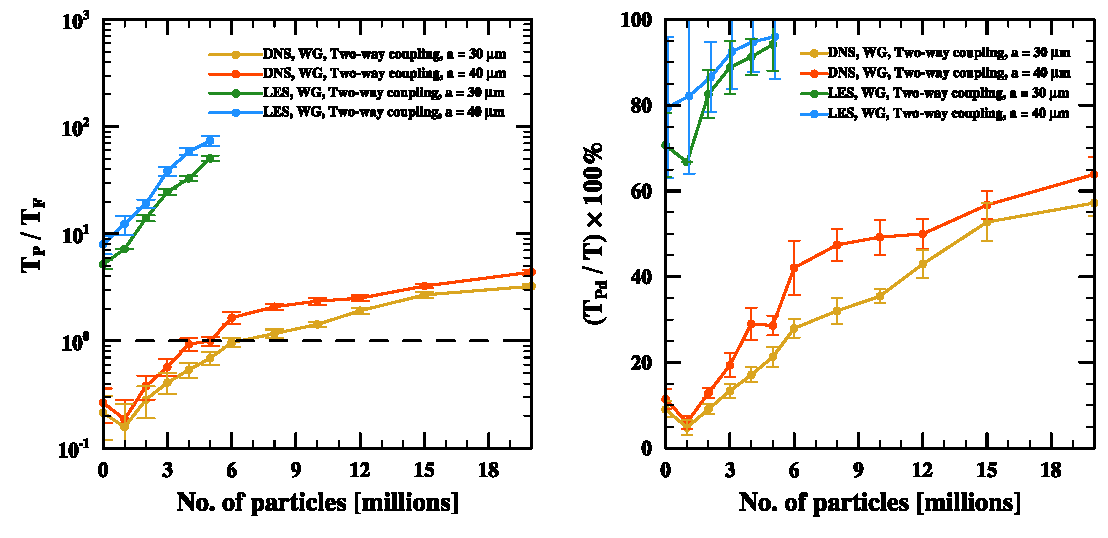
\includegraphics[width=13.5cm]{figures/3-10_pfftwcex.pdf}
\caption{
The ratio of average wall-clock times spent on processing particles, $T_{\text{P}}$, and the fluid flow, $T_{\text{F}}$ (left, linear-log scale); and average percentage of overall step time occupied by particle postprocessing tasks, $(T_{\text{Pd}} / T)$ (right).
Both statistics are shown for TWC simulations with gravity and.
Plots for LES on the right have slight horizontal offset added to make uncertainty bars more visible.
Consistent with Figure \ref{fig:pffowclesex}.
}
\label{fig:pfftwcex}
\end{figure}

% FIGURE 3-11 - TWC-SPECIFIC COMPUTATION TIMINGS FOR TWC SIMULATIONS
    
\begin{figure}
\centering
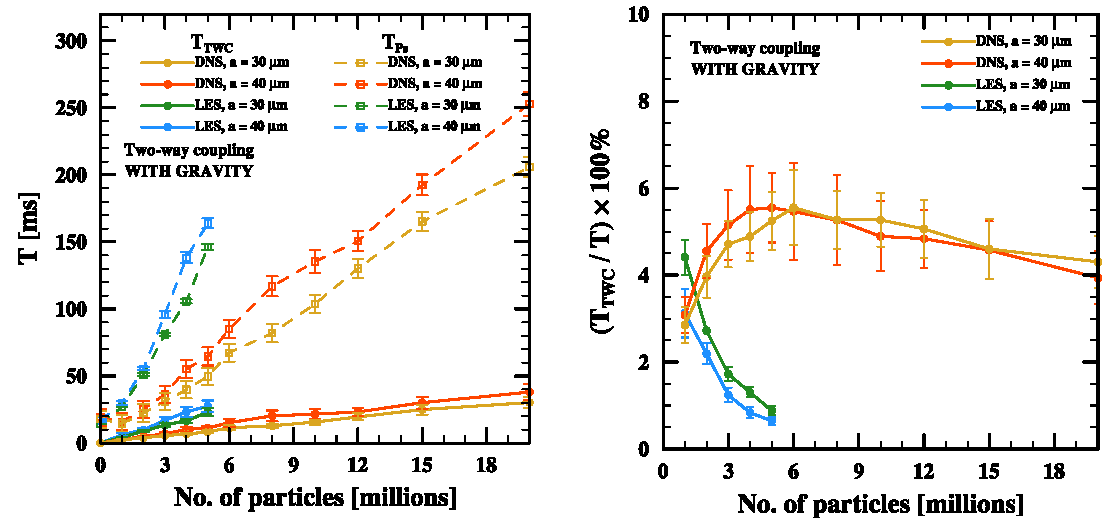
\includegraphics[width=13.5cm]{figures/3-11_pfftwctwc.pdf}
\caption{
Time- and process-averaged wall-clock times of TWC-specific stage, $T_{\text{TWC}}$, and all stages of the particle solver, $T_{\text{Ps}}$ (dashed line; left); and average percentage of $T_{\text{TWC}}$ as part of the entire step time, $T$.
All data is shown for TWC simulations with gravity and as a function of the number of particles in the system.
}
\label{fig:pfftwctwc}
\end{figure}

% FIGURE 3-12 - TIMINGS FOR INTERPROCESS COMMUNICATION

\begin{figure}
\centering
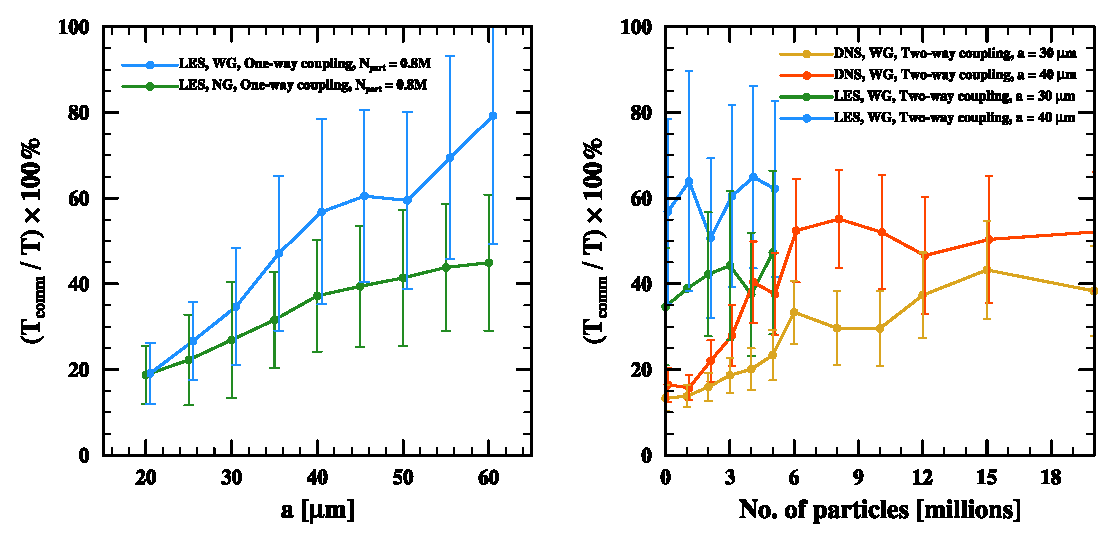
\includegraphics[width=13.5cm]{figures/3-12_pffcomm.pdf}
\caption{
Average percentage of wall-clock time per step spent on interprocess communications (excluding 3D FFT) for OWC LES (left) and TWC (right) simulations.
}
\label{fig:pffcomm}
\end{figure}
    
% FIGURE 3-13 - PARTICLE POSTPROCESSING TIMES DEPENDING ON RDF
    
\begin{figure}
\centering
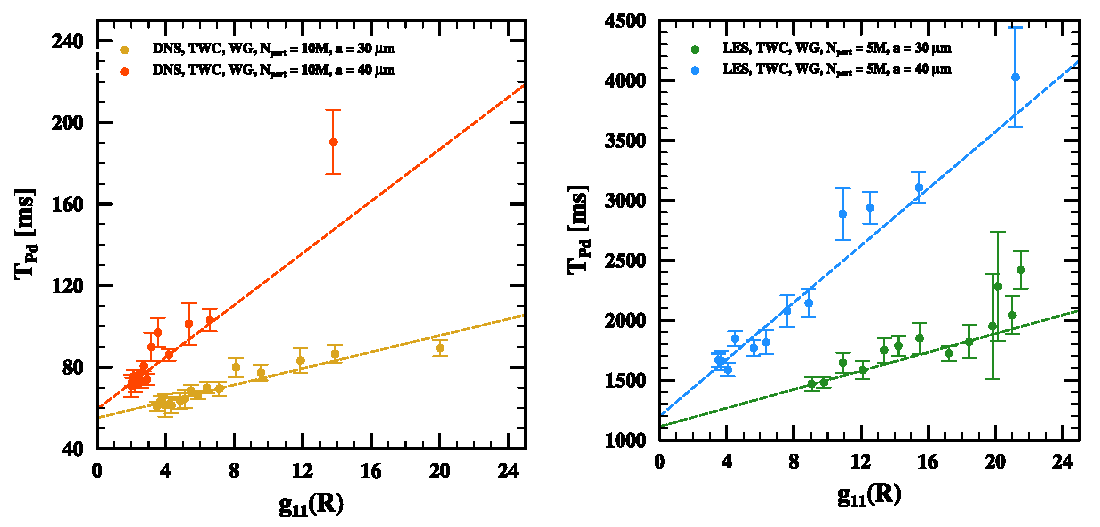
\includegraphics[width=13.5cm]{figures/3-13_pffrdfpd.pdf}
\caption{
Time- and process-averaged wall-clock times of particle postprocessing stage per step for DNS (left) and LES (right), depending on the estimated values of the radial distribution function at contact range (RDF at $r=R$).
Consistent with Figure \ref{fig:pfsrdf}.
}
\label{fig:pffrdfpd}
\end{figure}

% FIGURE 3-13 - PARTICLE SOLVER PROCESSING TIMES DEPENDING ON RDF

\begin{figure}
\centering
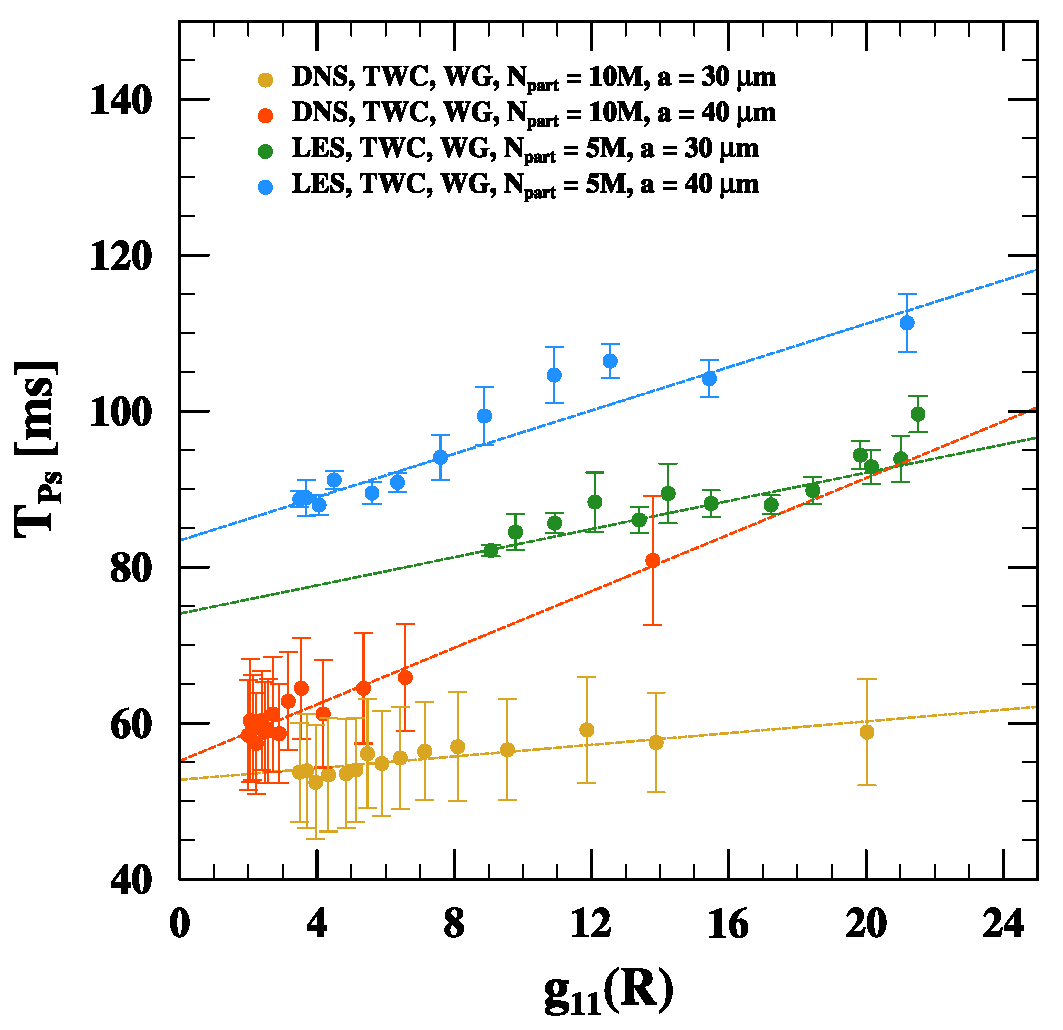
\includegraphics[width=8cm]{figures/3-14_pffrdfps.pdf}
\caption{
Time- and process-averaged wall-clock times of particle solver stages per step for DNS and LES, depending on the estimated values of the radial distribution function at contact range (RDF at $r=R$).
Consistent with Figure \ref{fig:pfsrdf}.
}
\label{fig:pffrdfps}
\end{figure}
    
% FIGURE 3-15 - CORRELATION BETWEEN RDF AND PARTICLE DISTRIBUTION IN SUBDOMAINS 

\begin{figure}
\centering
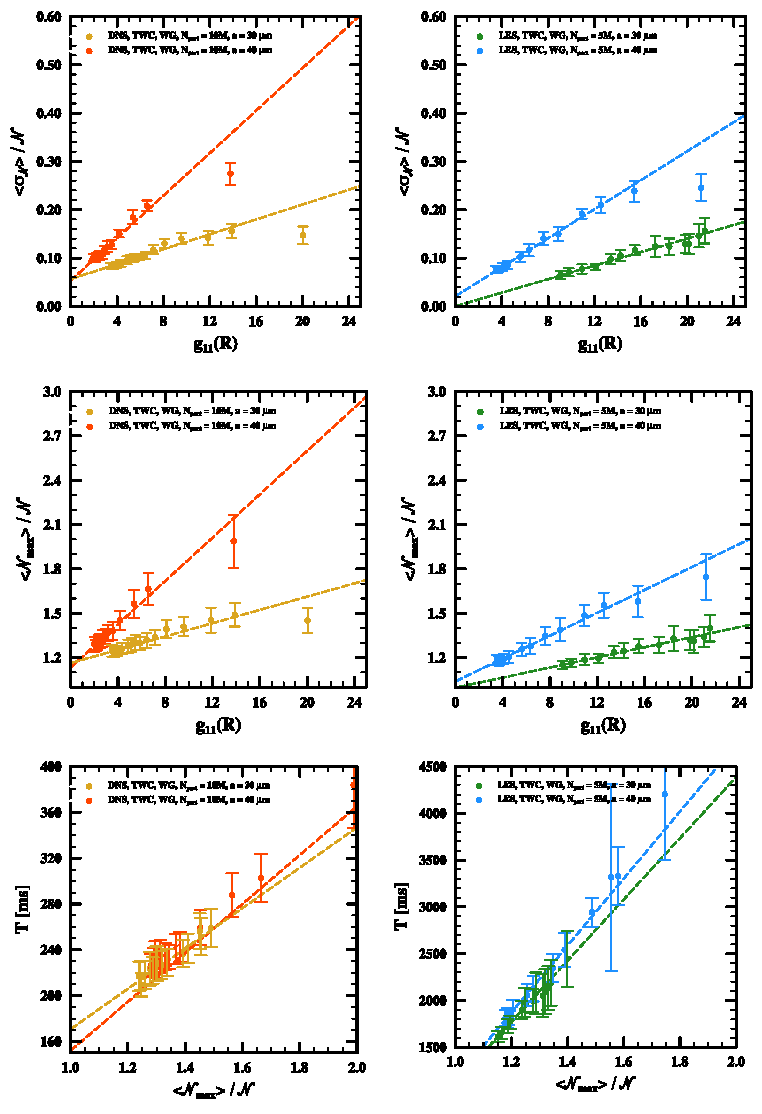
\includegraphics[width=13.5cm]{figures/3-15_pfprdf.pdf}
\caption{
Correlation between the RDF at contact distance and particle distribution statistics: time-averaged standard deviation, $\langle \sigma_{\mathcal{N}} \rangle$ (top), and maximal particle count, $\langle \mathcal{N}_{\max} \rangle$, normalised by average number of particles per subdomain for DNS (left) and LES (right).
Also correlation between normalised maximal particle counts and average total step times, $T$, is included (bottom).
Consistent with Figure \ref{fig:pfsrdf}.
}
\label{fig:pfprdf}
\end{figure}

% FIGURE 3-16 - PARTICLE DISTRIBUTION IN SUBDOMAINS IN TWC

\begin{figure}
\centering
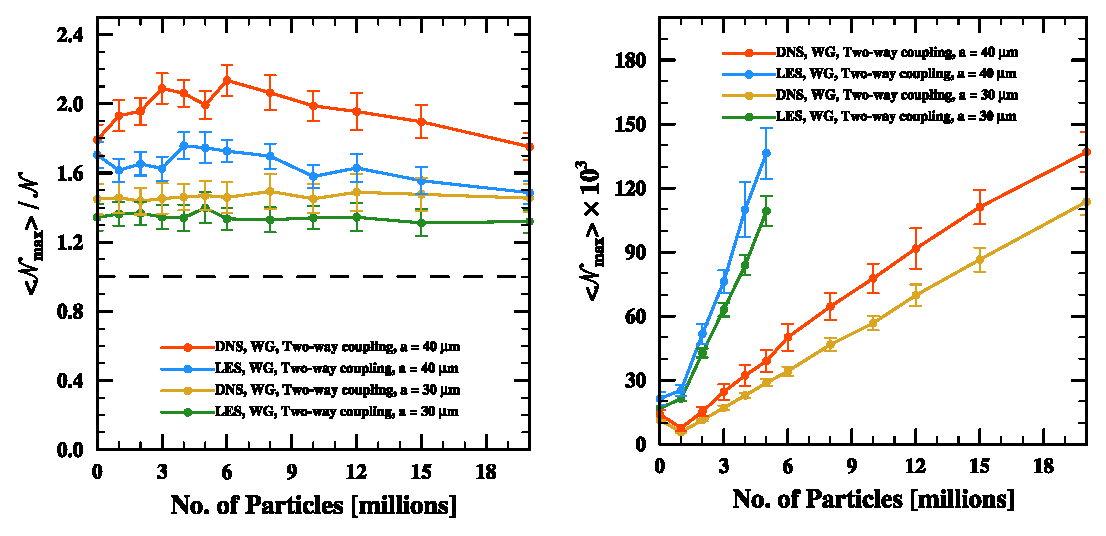
\includegraphics[width=13.5cm]{figures/3-16_pfptwc.pdf}
\caption{
Time-averaged maximal number of particles in subdomains, $\langle \mathcal{N}_{\max} \rangle$, for TWC simulations with gravity (DNS and LES).
On the left, values are normalised by the average number of particles per subdomain; on the right, absolute values are given (in thousands of particles).
}
\label{fig:pfptwc}
\end{figure}

% FIGURE 3-17 - PARTICLE DISTRIBUTION IN SUBDOMAINS IN OWC

\begin{figure}
\centering
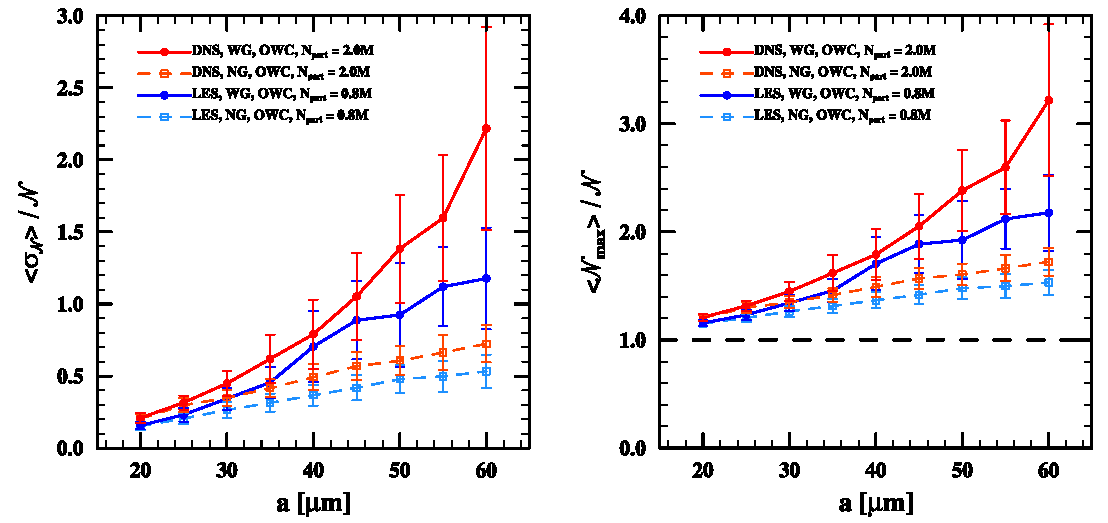
\includegraphics[width=13.5cm]{figures/3-17_pfpowc.pdf}
\caption{
Time-averaged standard deviation, $\langle \sigma(\mathcal{N}) \rangle$ (left), and maximal number of particles in~subdomains, $\langle \mathcal{N}_{\max} \rangle$ (right), for OWC simulations with and without gravity (DNS and LES).
Values are normalised by the average number of particles per subdomain.
}
\label{fig:pfpowc}
\end{figure}
    
% FIGURE 3-18 - GRID FOR PARTICLE DISTRIBUTION IN SUBDOMAINS (MAX) IN OWC

\begin{figure}
\centering
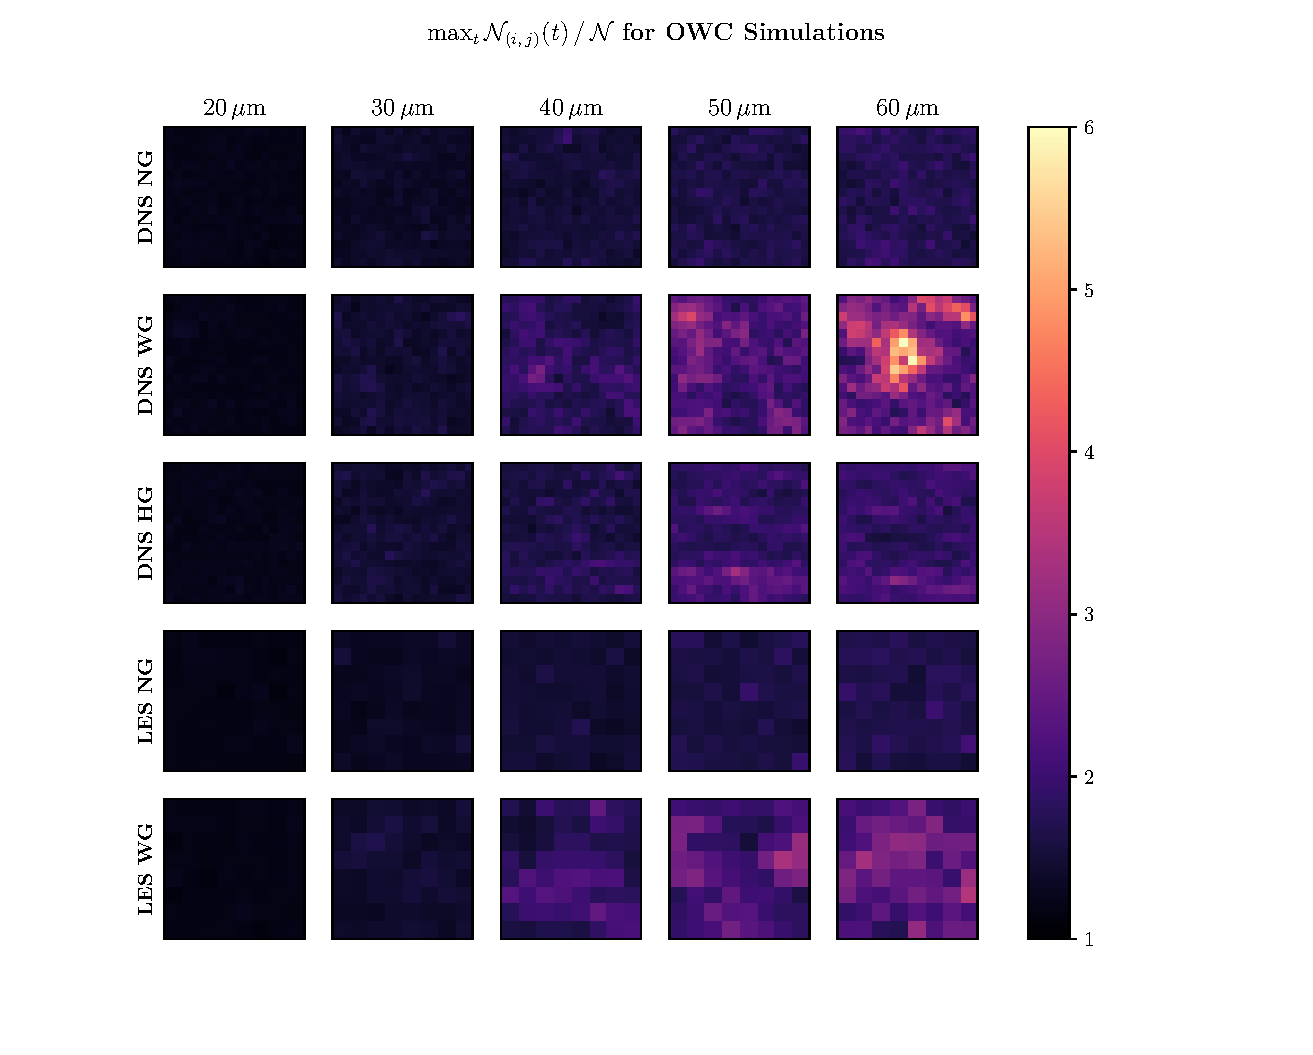
\includegraphics[width=17cm]{figures/3-18_pfpgridowcmax.pdf}
\caption{
Maximum number of particles for every subdomain taken over the entire run for OWC simulations with droplets of different radii.
Results are included for both DNS and LES: NG -- without gravity, WG -- with gravity; HG -- with ``horizontal'' gravity (i.e. pointing perpendicular to the domain boundaries).
Values are normalised by the average number of particles per subdomain.
}
\label{fig:pfpgridowcmax}
\end{figure}    

% FIGURE 3-19 - GRID FOR PARTICLE DISTRIBUTION IN SUBDOMAINS (STANDARD DEVIATION) IN OWC

\begin{figure}
\centering
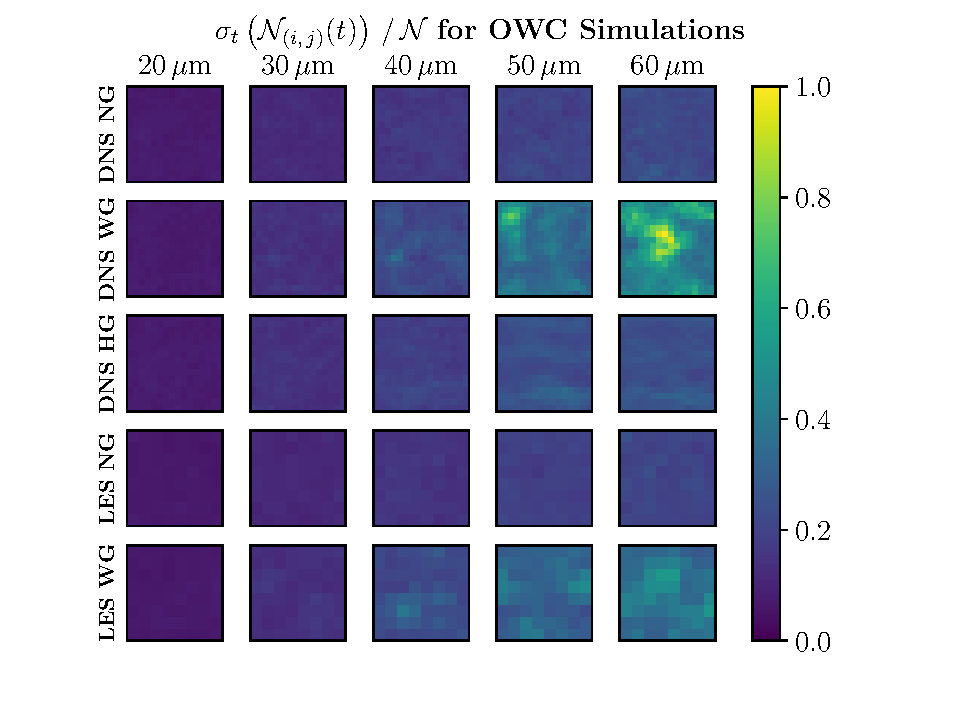
\includegraphics[width=13.5cm]{figures/3-19_pfpgridowcstd.pdf}
\caption{
Standard deviation of particle counts for every subdomain taken over the entire run for OWC simulations with droplets of different radii.
Consistent with Figure \ref{fig:pfpgridowcstd}.
}
\label{fig:pfpgridowcstd}
\end{figure}    

% FIGURE 3-20 - GRID FOR PARTICLE DISTRIBUTION IN SUBDOMAINS (ACTUAL - LAST STEP) IN OWC

\begin{figure}
\centering
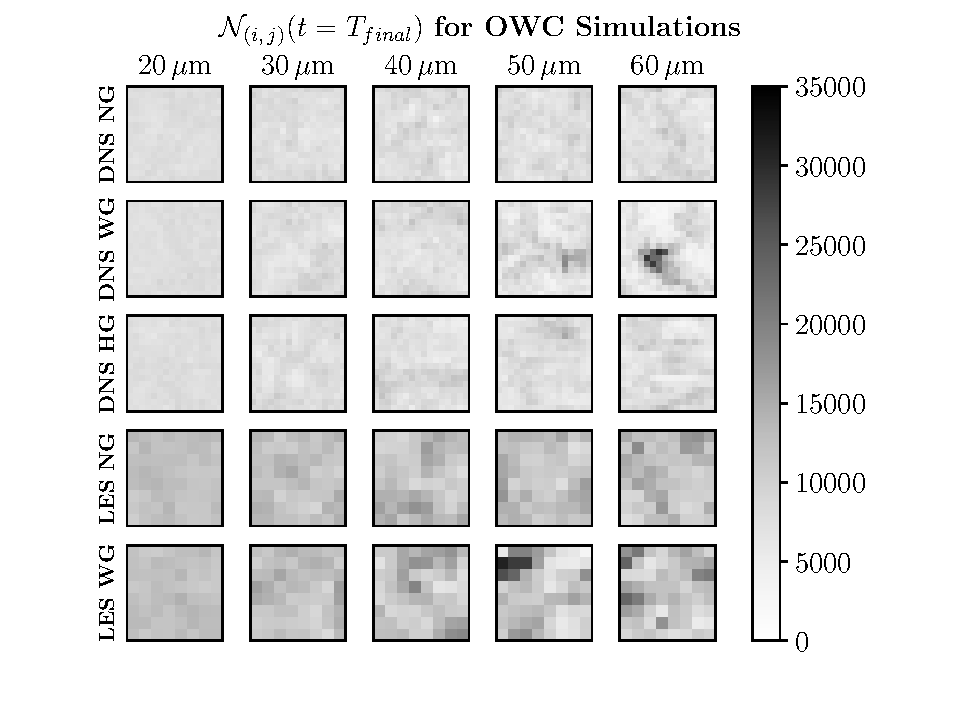
\includegraphics[width=13.5cm]{figures/3-20_pfpgridowclast.pdf}
\caption{
Particle counts for every subdomain taken from the last processed time step for OWC simulations with droplets of different radii.
Average number of particles per subdomain are: $7 812.5$ for DNS, $12 500$ for LES.
Consistent with Figure \ref{fig:pfpgridowcstd}.
}
\label{fig:pfpgridowclast}
\end{figure}

% FIGURE 3-21 - HORIZONTAL GRAVITY IN OWC - PERFORMANCE COMPARISON

\begin{figure}
\centering
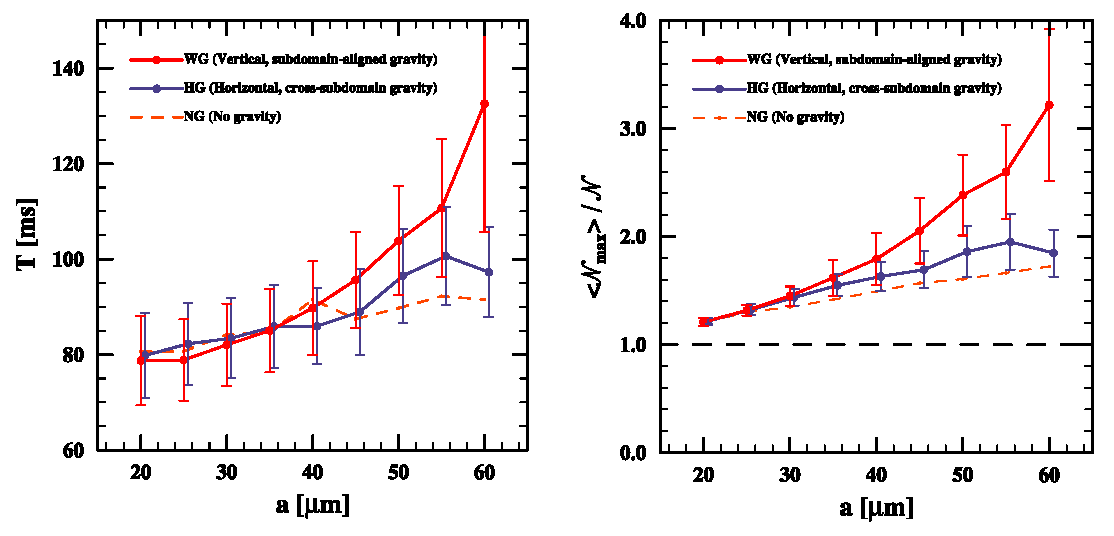
\includegraphics[width=13.5cm]{figures/3-21_howcperf.pdf}
\caption{
Time-averaged wall-clock times per step, $T$ (left), and normalised maximal number of particles in subdomains, $(\langle \mathcal{N}_{\max} \rangle / \mathcal{N})$ (right) for DNS simulations under one-way momentum coupling (OWC) with different directions of gravity (relative to the direction of domain decomposition).
Results of simulations without gravity are shown with dashed lines for comparison. 
}
\label{fig:howcperf}
\end{figure}
    
% FIGURE 3-22 - HORIZONTAL GRAVITY IN OWC - PHYSICAL FIDELITY COMPARISON (RDF AND RRV)

\begin{figure}
\centering
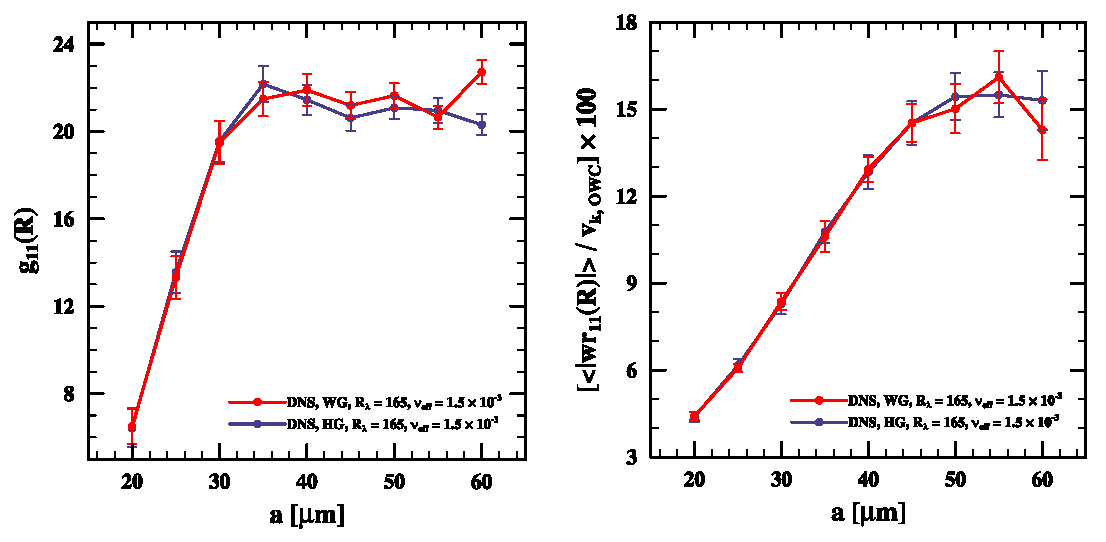
\includegraphics[width=13.5cm]{figures/3-22_howcrdfrrv.pdf}
\caption{
The values of the radial distribution function (RDF, left) and the radial relative velocity (RRV, right) at contact distance for simulations with one-way momentum coupling.
Results include data from DNS simulations with different directions of gravity vector (relative to the direction of domain decomposition).
}
\label{fig:howcrdfrrv}
\end{figure}
    
% FIGURE 3-23 - GRID FOR PARTICLE DISTRIBUTION IN SUBDOMAINS (MAX) IN TWC

\begin{figure}
\centering
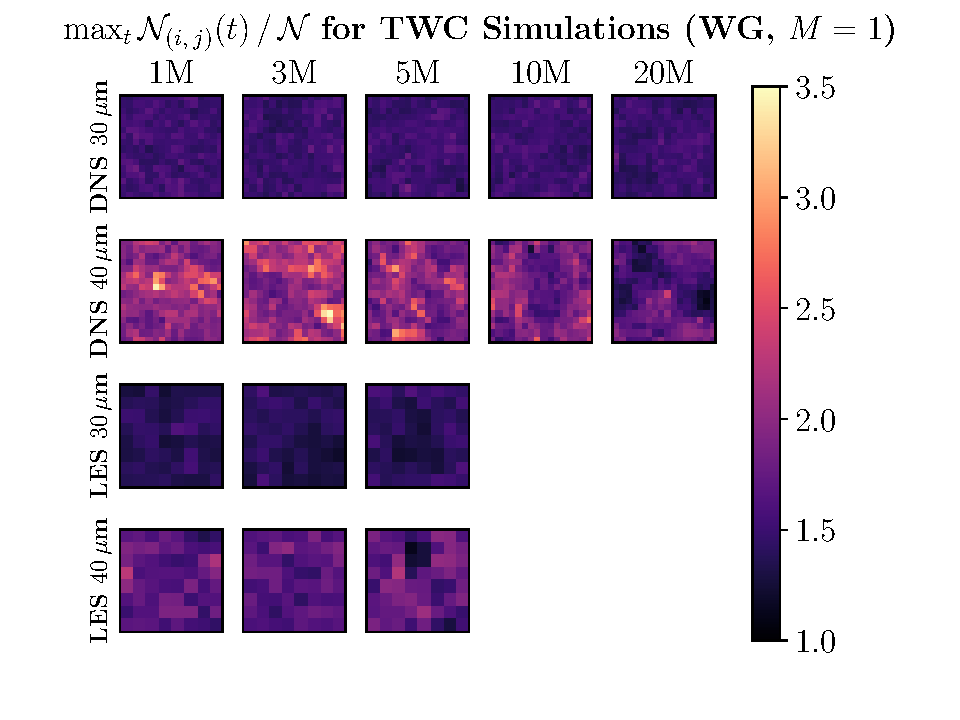
\includegraphics[width=10cm]{figures/3-23_pfpgridtwcmax.pdf}
\caption{
Maximum number of particles for every subdomain taken over the entire run for TWC simulations with gravity and radii $30$, $40$~$\upmu\text{m}$.
All simulations were conducted without superparticle parameterisation ($M=1$). 
Values are normalised by the average number of particles per subdomain.
Consistent with Figure \ref{fig:pfpgridowcmax}.
}
\label{fig:pfpgridtwcmax}
\end{figure}    

% FIGURE 3-24 - GRID FOR PARTICLE DISTRIBUTION IN SUBDOMAINS (STANDARD DEVIATION) IN TWC WITH HIGH MASS LOADINGS

\begin{figure}
\centering
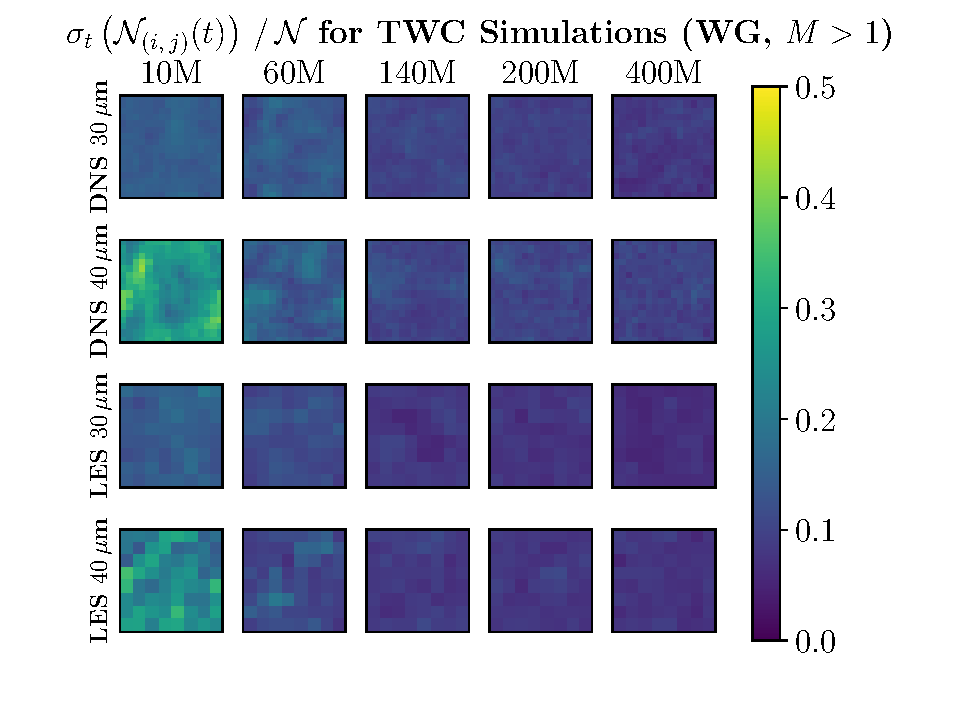
\includegraphics[width=10cm]{figures/3-24_pfpgridrdfstd.pdf}
\caption{
Standard deviation of particle counts for every subdomain taken over the entire run for TWC simulations with gravity and radii $30$, $40$~$\upmu\text{m}$.
All simulations were conducted with superparticle parameterisation ($M>1$). 
Values are normalised by the average number of particles per subdomain.
Consistent with Figure \ref{fig:pfpgridowcstd}.
}
\label{fig:pfpgridrdfstd}
\end{figure}

 

%%% ==================== %%%
%%%      APPENDIX B      %%%
%%% ==================== %%%

% FIGURE B-01 - ENERGY SCECTRA FOR DIFFERENT VALUES OF SGS PARAMETER C_K

\begin{figure}
\centering
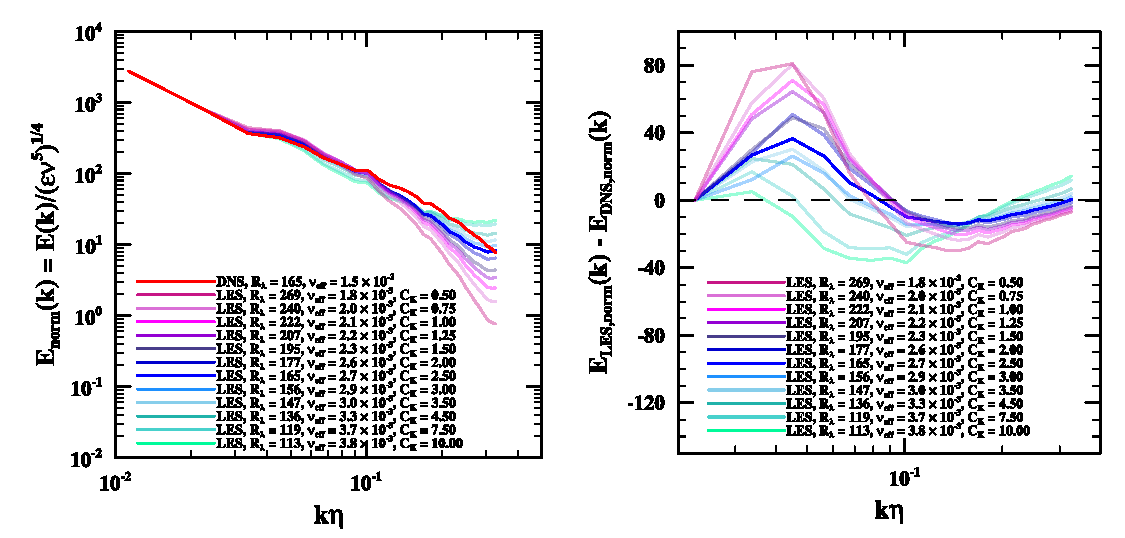
\includegraphics[width=13.5cm]{figures/B-01_sgsspec.pdf}
\caption{
The normalised energy spectra of background turbulent flows for LES for different values of the subgrid-scale model parameter $C_K$. 
On the left, respective spectra are shown with reference DNS spectrum shown in red (log-log scale).
On the right, for more clarity, plot of differences between respective LES spectra and reference DNS spectrum is presented (log-linear scale).
Spectrum for LES used in this thesis (with $C_K=2.5$) is marked with bolder, more vivid shade of blue.
}
\label{fig:sgsspec}
\end{figure}